\section{Background and data yields }

We will not repeat yields and data/MC control plots from the control region in this note. The corresponding information can be found in Sec. 9 of ~\cite{alphaTnote}. Distributions and yield are presented for all three jet selections (monojet, asymmetric and symmetric selection) and various distributions (jet multiplicities, \ht, \htmiss, object $p_\textrm{T}$, angular variables).

In the absence of multijet events from QCD the remaining backgrounds in the signal region are expected to stem from SM processes with genuine \met in the final state. For the low jet multiplicity categories, the largest backgrounds with \met are from the associated production of $$W or $Z$ bosons with jets, followed by either the weak decays \znunu\ or \wtaunu, where the $\tau$ decays hadronically and is identified as a jet, or by leptonic decays that are outside acceptance or not rejected by the dedicated electron or muon vetoes. For the higher jet multiplicity categories, semileptonic decaying top quark production becomes dominant. The relative contribution from \ttbar depends on the jet multiplicity with increase importance for large jet multiplicities.




%Tables~\ref{tab:prednodata_sig_comb_sym},
%\ref{tab:prednodata_sig_comb_asym} and \ref{tab:prednodata_sig_comb_mono} 
%summarise the predicted pre-fit yields and uncertainties in the signal region for an integrated
%luminosity of 1.28 \ifb. In addition to the total expected yield (SM) per (\njet,~\nb,~\scalht) bin, the $\ttbar$W and \znunu\ contributions
%are also shown (the former of which contains all residual contributions from sub-dominant processes such as \eg diboson
%production).
%\clearpage
%\begin{table}[h!]
\tiny
\centering
\caption{Pre fit Yields in the signal region for 2.1\ifb for symmetric categories. All entries are non-zero but are truncated to one decimal place.\label{tab:prednodata_sig_comb_sym}}
\begin{tabular}
{cccccccccc}
	\hline\hline
	&	& \multicolumn{8}{c}{\scalht (\gev)}\\ 
	&	 (\njet, \nb) & 200-250 & 250-300 & 300-350 & 350-400 & 400-500 & 500-600 & 600-800 & 800-$\infty$ \\ [0.8ex] 
\hline
	SM & (2, 0) & $943.9^{+ 134.2 }_{- 134.2 }$ & $938.4^{+ 148.4 }_{- 148.4 }$ & $627.9^{+ 86.0 }_{- 86.0 }$ & $341.4^{+ 61.3 }_{- 61.3 }$ & $329.1^{+ 38.4 }_{- 38.4 }$ & $105.2^{+ 24.3 }_{- 24.3 }$ & $43.8^{+ 12.2 }_{- 12.2 }$ & $44.4^{+ 11.4 }_{- 11.4 }$ \\[0.5ex] 
	Ttw & (2, 0) & $425.8^{+ 84.5 }_{- 84.5 }$ & $415.9^{+ 81.1 }_{- 81.1 }$ & $262.5^{+ 41.1 }_{- 41.1 }$ & $128.7^{+ 24.8 }_{- 24.8 }$ & $113.1^{+ 12.9 }_{- 12.9 }$ & $33.0^{+ 9.1 }_{- 9.1 }$ & $13.3^{+ 2.7 }_{- 2.7 }$ & $12.8^{+ 2.8 }_{- 2.8 }$ \\[0.5ex] 
	Zinv & (2, 0) & $457.5^{+ 86.4 }_{- 86.4 }$ & $517.5^{+ 116.8 }_{- 116.8 }$ & $353.5^{+ 63.8 }_{- 63.8 }$ & $210.4^{+ 50.0 }_{- 50.0 }$ & $206.4^{+ 28.1 }_{- 28.1 }$ & $67.7^{+ 18.5 }_{- 18.5 }$ & $30.4^{+ 11.0 }_{- 11.0 }$ & $31.2^{+ 9.5 }_{- 9.5 }$ \\[0.5ex] 
	SM & (2, 1) & $80.9^{+ 16.0 }_{- 16.0 }$ & $57.9^{+ 11.1 }_{- 11.1 }$ & $40.8^{+ 7.3 }_{- 7.3 }$ & $26.8^{+ 5.7 }_{- 5.7 }$ & $24.1^{+ 3.7 }_{- 3.7 }$ & $9.5^{+ 2.7 }_{- 2.7 }$ & $4.0^{+ 1.4 }_{- 1.4 }$ & $3.7^{+ 1.3 }_{- 1.3 }$ \\[0.5ex] 
	Ttw & (2, 1) & $50.5^{+ 12.8 }_{- 12.8 }$ & $33.7^{+ 7.4 }_{- 7.4 }$ & $20.3^{+ 4.2 }_{- 4.2 }$ & $11.0^{+ 2.6 }_{- 2.6 }$ & $8.4^{+ 1.3 }_{- 1.3 }$ & $2.9^{+ 1.0 }_{- 1.0 }$ & $1.0^{+ 0.3 }_{- 0.3 }$ & $1.0^{+ 0.3 }_{- 0.3 }$ \\[0.5ex] 
	Zinv & (2, 1) & $25.2^{+ 6.0 }_{- 6.0 }$ & $23.9^{+ 5.9 }_{- 5.9 }$ & $19.8^{+ 4.3 }_{- 4.3 }$ & $15.7^{+ 4.0 }_{- 4.0 }$ & $14.9^{+ 2.5 }_{- 2.5 }$ & $6.2^{+ 2.0 }_{- 2.0 }$ & $3.0^{+ 1.2 }_{- 1.2 }$ & $2.6^{+ 1.0 }_{- 1.0 }$ \\[0.5ex] 
	SM & (2, 2) & $1.1^{+ 2.3 }_{- 2.3 }$ & $0.8^{+ 1.9 }_{- 1.9 }$ & $3.4^{+ 2.0 }_{- 2.0 }$ & $0.7^{+ 0.8 }_{- 0.8 }$ & $1.1^{+ 0.5 }_{- 0.5 }$ & $1.3^{+ 0.8 }_{- 0.8 }$ & $0.2^{+ 0.2 }_{- 0.2 }$ & -- \\[0.5ex] 
	Ttw & (2, 2) & $0.5^{+ 1.2 }_{- 1.2 }$ & $0.4^{+ 0.9 }_{- 0.9 }$ & $1.7^{+ 1.0 }_{- 1.0 }$ & $0.3^{+ 0.3 }_{- 0.3 }$ & $0.4^{+ 0.2 }_{- 0.2 }$ & $0.8^{+ 0.6 }_{- 0.6 }$ & $0.1^{+ 0.0 }_{- 0.0 }$ & -- \\[0.5ex] 
	Zinv & (2, 2) & $0.5^{+ 1.1 }_{- 1.1 }$ & $0.4^{+ 1.0 }_{- 1.0 }$ & $1.6^{+ 1.0 }_{- 1.0 }$ & $0.4^{+ 0.4 }_{- 0.4 }$ & $0.6^{+ 0.3 }_{- 0.3 }$ & $0.4^{+ 0.2 }_{- 0.2 }$ & $0.1^{+ 0.1 }_{- 0.1 }$ & -- \\[0.5ex] 
	SM & (3, 0) & $0.0^{+ 2.4 }_{- 2.4 }$ & $173.6^{+ 26.2 }_{- 26.2 }$ & $491.8^{+ 63.6 }_{- 63.6 }$ & $421.9^{+ 58.6 }_{- 58.6 }$ & $499.2^{+ 65.1 }_{- 65.1 }$ & $195.4^{+ 36.8 }_{- 36.8 }$ & $89.5^{+ 23.7 }_{- 23.7 }$ & $68.0^{+ 11.6 }_{- 11.6 }$ \\[0.5ex] 
	Ttw & (3, 0) & $0.0^{+ 1.9 }_{- 1.9 }$ & $80.3^{+ 12.6 }_{- 12.6 }$ & $237.0^{+ 35.4 }_{- 35.4 }$ & $190.6^{+ 27.4 }_{- 27.4 }$ & $207.0^{+ 32.1 }_{- 32.1 }$ & $68.1^{+ 14.1 }_{- 14.1 }$ & $29.1^{+ 5.3 }_{- 5.3 }$ & $18.1^{+ 3.6 }_{- 3.6 }$ \\[0.5ex] 
	Zinv & (3, 0) & $0.0^{+ 0.6 }_{- 0.6 }$ & $90.9^{+ 19.9 }_{- 19.9 }$ & $243.3^{+ 47.7 }_{- 47.7 }$ & $212.9^{+ 38.9 }_{- 38.9 }$ & $282.4^{+ 44.2 }_{- 44.2 }$ & $111.6^{+ 25.2 }_{- 25.2 }$ & $60.4^{+ 21.2 }_{- 21.2 }$ & $45.4^{+ 8.8 }_{- 8.8 }$ \\[0.5ex] 
	SM & (3, 1) & -- & $37.9^{+ 6.3 }_{- 6.3 }$ & $70.5^{+ 11.1 }_{- 11.1 }$ & $81.2^{+ 11.9 }_{- 11.9 }$ & $79.2^{+ 11.6 }_{- 11.6 }$ & $26.4^{+ 5.9 }_{- 5.9 }$ & $15.3^{+ 4.1 }_{- 4.1 }$ & $9.2^{+ 2.0 }_{- 2.0 }$ \\[0.5ex] 
	Ttw & (3, 1) & -- & $29.3^{+ 5.2 }_{- 5.2 }$ & $51.3^{+ 9.6 }_{- 9.6 }$ & $54.3^{+ 8.1 }_{- 8.1 }$ & $47.4^{+ 7.9 }_{- 7.9 }$ & $13.0^{+ 3.3 }_{- 3.3 }$ & $5.9^{+ 1.2 }_{- 1.2 }$ & $2.7^{+ 0.7 }_{- 0.7 }$ \\[0.5ex] 
	Zinv & (3, 1) & -- & $8.1^{+ 2.0 }_{- 2.0 }$ & $17.6^{+ 3.7 }_{- 3.7 }$ & $23.4^{+ 5.1 }_{- 5.1 }$ & $30.2^{+ 5.6 }_{- 5.6 }$ & $11.2^{+ 3.0 }_{- 3.0 }$ & $9.4^{+ 3.5 }_{- 3.5 }$ & $5.9^{+ 1.5 }_{- 1.5 }$ \\[0.5ex] 
	SM & (3, 2) & -- & $5.9^{+ 1.7 }_{- 1.7 }$ & $17.5^{+ 3.2 }_{- 3.2 }$ & $16.4^{+ 3.0 }_{- 3.0 }$ & $11.3^{+ 2.2 }_{- 2.2 }$ & $3.4^{+ 1.0 }_{- 1.0 }$ & $0.8^{+ 0.3 }_{- 0.3 }$ & $0.9^{+ 0.3 }_{- 0.3 }$ \\[0.5ex] 
	Ttw & (3, 2) & -- & $4.7^{+ 1.4 }_{- 1.4 }$ & $14.3^{+ 2.8 }_{- 2.8 }$ & $13.5^{+ 2.7 }_{- 2.7 }$ & $8.5^{+ 1.8 }_{- 1.8 }$ & $2.0^{+ 0.6 }_{- 0.6 }$ & $0.2^{+ 0.1 }_{- 0.1 }$ & $0.3^{+ 0.1 }_{- 0.1 }$ \\[0.5ex] 
	Zinv & (3, 2) & -- & $1.2^{+ 0.4 }_{- 0.4 }$ & $2.8^{+ 0.6 }_{- 0.6 }$ & $2.2^{+ 0.5 }_{- 0.5 }$ & $2.7^{+ 0.6 }_{- 0.6 }$ & $1.1^{+ 0.4 }_{- 0.4 }$ & $0.5^{+ 0.2 }_{- 0.2 }$ & $0.6^{+ 0.2 }_{- 0.2 }$ \\[0.5ex] 
	SM & (3, $\ge3$) & -- & $0.0^{+ 0.3 }_{- 0.3 }$ & -- & -- & $0.4^{+ 0.2 }_{- 0.2 }$ & -- & -- & -- \\[0.5ex] 
	Ttw & (3, $\ge3$) & -- & $0.0^{+ 0.3 }_{- 0.3 }$ & -- & -- & $0.3^{+ 0.2 }_{- 0.2 }$ & -- & -- & -- \\[0.5ex] 
	Zinv & (3, $\ge3$) & -- & $0.0^{+ 0.0 }_{- 0.0 }$ & -- & -- & $0.1^{+ 0.0 }_{- 0.0 }$ & -- & -- & -- \\[0.5ex] 
	SM & (4, 0) & -- & -- & $48.8^{+ 14.1 }_{- 14.1 }$ & $163.1^{+ 65.7 }_{- 65.7 }$ & $301.0^{+ 46.9 }_{- 46.9 }$ & $155.8^{+ 36.3 }_{- 36.3 }$ & $96.5^{+ 19.1 }_{- 19.1 }$ & $52.8^{+ 11.3 }_{- 11.3 }$ \\[0.5ex] 
	Ttw & (4, 0) & -- & -- & $27.7^{+ 10.0 }_{- 10.0 }$ & $87.3^{+ 27.6 }_{- 27.6 }$ & $150.8^{+ 19.9 }_{- 19.9 }$ & $62.9^{+ 15.6 }_{- 15.6 }$ & $35.4^{+ 7.6 }_{- 7.6 }$ & $17.3^{+ 4.5 }_{- 4.5 }$ \\[0.5ex] 
	Zinv & (4, 0) & -- & -- & $20.6^{+ 8.0 }_{- 8.0 }$ & $74.8^{+ 54.5 }_{- 54.5 }$ & $150.2^{+ 36.3 }_{- 36.3 }$ & $88.5^{+ 27.6 }_{- 27.6 }$ & $60.7^{+ 13.5 }_{- 13.5 }$ & $35.5^{+ 8.3 }_{- 8.3 }$ \\[0.5ex] 
	SM & (4, 1) & -- & -- & $19.9^{+ 6.3 }_{- 6.3 }$ & $67.1^{+ 19.0 }_{- 19.0 }$ & $84.6^{+ 11.7 }_{- 11.7 }$ & $36.9^{+ 8.3 }_{- 8.3 }$ & $18.4^{+ 4.3 }_{- 4.3 }$ & $11.6^{+ 2.5 }_{- 2.5 }$ \\[0.5ex] 
	Ttw & (4, 1) & -- & -- & $17.0^{+ 6.0 }_{- 6.0 }$ & $55.4^{+ 16.3 }_{- 16.3 }$ & $65.5^{+ 9.0 }_{- 9.0 }$ & $23.4^{+ 6.0 }_{- 6.0 }$ & $9.9^{+ 2.6 }_{- 2.6 }$ & $4.7^{+ 1.2 }_{- 1.2 }$ \\[0.5ex] 
	Zinv & (4, 1) & -- & -- & $2.7^{+ 1.1 }_{- 1.1 }$ & $11.3^{+ 8.9 }_{- 8.9 }$ & $19.0^{+ 4.9 }_{- 4.9 }$ & $12.5^{+ 3.7 }_{- 3.7 }$ & $8.5^{+ 2.1 }_{- 2.1 }$ & $6.9^{+ 1.6 }_{- 1.6 }$ \\[0.5ex] 
	SM & (4, 2) & -- & -- & $3.6^{+ 2.0 }_{- 2.0 }$ & $17.2^{+ 5.8 }_{- 5.8 }$ & $31.9^{+ 5.0 }_{- 5.0 }$ & $7.3^{+ 2.1 }_{- 2.1 }$ & $2.8^{+ 0.7 }_{- 0.7 }$ & $2.1^{+ 0.6 }_{- 0.6 }$ \\[0.5ex] 
	Ttw & (4, 2) & -- & -- & $3.2^{+ 1.9 }_{- 1.9 }$ & $16.2^{+ 5.7 }_{- 5.7 }$ & $28.5^{+ 4.6 }_{- 4.6 }$ & $5.9^{+ 1.8 }_{- 1.8 }$ & $1.7^{+ 0.4 }_{- 0.4 }$ & $1.1^{+ 0.4 }_{- 0.4 }$ \\[0.5ex] 
	Zinv & (4, 2) & -- & -- & $0.4^{+ 0.2 }_{- 0.2 }$ & $0.9^{+ 0.6 }_{- 0.6 }$ & $3.4^{+ 0.9 }_{- 0.9 }$ & $1.2^{+ 0.4 }_{- 0.4 }$ & $1.0^{+ 0.3 }_{- 0.3 }$ & $1.0^{+ 0.3 }_{- 0.3 }$ \\[0.5ex] 
	SM & (4, $\ge3$) & -- & -- & $0.0^{+ 0.4 }_{- 0.4 }$ & $1.5^{+ 1.1 }_{- 1.1 }$ & $1.5^{+ 0.8 }_{- 0.8 }$ & $0.6^{+ 0.4 }_{- 0.4 }$ & $0.0^{+ 0.1 }_{- 0.1 }$ & $0.0^{+ 0.0 }_{- 0.0 }$ \\[0.5ex] 
	Ttw & (4, $\ge3$) & -- & -- & $0.0^{+ 0.4 }_{- 0.4 }$ & $1.3^{+ 1.0 }_{- 1.0 }$ & $1.4^{+ 0.7 }_{- 0.7 }$ & $0.5^{+ 0.3 }_{- 0.3 }$ & $0.0^{+ 0.0 }_{- 0.0 }$ & $0.0^{+ 0.0 }_{- 0.0 }$ \\[0.5ex] 
	Zinv & (4, $\ge3$) & -- & -- & $0.0^{+ 0.0 }_{- 0.0 }$ & $0.1^{+ 0.2 }_{- 0.2 }$ & $0.1^{+ 0.1 }_{- 0.1 }$ & $0.1^{+ 0.1 }_{- 0.1 }$ & $0.0^{+ 0.0 }_{- 0.0 }$ & $0.0^{+ 0.0 }_{- 0.0 }$ \\[0.5ex] 
	SM & ($\ge5$, 0) & -- & -- & -- & $15.3^{+ 5.9 }_{- 5.9 }$ & $86.1^{+ 13.1 }_{- 13.1 }$ & $78.1^{+ 20.0 }_{- 20.0 }$ & $71.0^{+ 14.4 }_{- 14.4 }$ & $46.2^{+ 12.8 }_{- 12.8 }$ \\[0.5ex] 
	Ttw & ($\ge5$, 0) & -- & -- & -- & $10.5^{+ 4.9 }_{- 4.9 }$ & $49.9^{+ 8.9 }_{- 8.9 }$ & $37.3^{+ 9.8 }_{- 9.8 }$ & $32.4^{+ 6.9 }_{- 6.9 }$ & $17.0^{+ 4.1 }_{- 4.1 }$ \\[0.5ex] 
	Zinv & ($\ge5$, 0) & -- & -- & -- & $4.7^{+ 1.4 }_{- 1.4 }$ & $32.8^{+ 7.5 }_{- 7.5 }$ & $36.1^{+ 11.8 }_{- 11.8 }$ & $37.4^{+ 9.6 }_{- 9.6 }$ & $28.1^{+ 10.4 }_{- 10.4 }$ \\[0.5ex] 
	SM & ($\ge5$, 1) & -- & -- & -- & $2.5^{+ 1.5 }_{- 1.5 }$ & $44.1^{+ 8.0 }_{- 8.0 }$ & $38.9^{+ 8.7 }_{- 8.7 }$ & $25.3^{+ 5.6 }_{- 5.6 }$ & $15.8^{+ 3.5 }_{- 3.5 }$ \\[0.5ex] 
	Ttw & ($\ge5$, 1) & -- & -- & -- & $2.2^{+ 1.4 }_{- 1.4 }$ & $37.4^{+ 7.4 }_{- 7.4 }$ & $30.8^{+ 7.3 }_{- 7.3 }$ & $18.5^{+ 4.6 }_{- 4.6 }$ & $9.9^{+ 2.3 }_{- 2.3 }$ \\[0.5ex] 
	Zinv & ($\ge5$, 1) & -- & -- & -- & $0.3^{+ 0.1 }_{- 0.1 }$ & $5.0^{+ 1.3 }_{- 1.3 }$ & $5.8^{+ 2.0 }_{- 2.0 }$ & $6.3^{+ 1.7 }_{- 1.7 }$ & $5.6^{+ 1.9 }_{- 1.9 }$ \\[0.5ex] 
	SM & ($\ge5$, 2) & -- & -- & -- & $2.1^{+ 1.3 }_{- 1.3 }$ & $18.8^{+ 4.1 }_{- 4.1 }$ & $15.4^{+ 3.8 }_{- 3.8 }$ & $7.6^{+ 1.9 }_{- 1.9 }$ & $4.6^{+ 1.2 }_{- 1.2 }$ \\[0.5ex] 
	Ttw & ($\ge5$, 2) & -- & -- & -- & $2.0^{+ 1.3 }_{- 1.3 }$ & $17.3^{+ 4.0 }_{- 4.0 }$ & $13.2^{+ 3.5 }_{- 3.5 }$ & $6.4^{+ 1.7 }_{- 1.7 }$ & $3.6^{+ 1.0 }_{- 1.0 }$ \\[0.5ex] 
	Zinv & ($\ge5$, 2) & -- & -- & -- & $0.1^{+ 0.1 }_{- 0.1 }$ & $0.8^{+ 0.3 }_{- 0.3 }$ & $1.3^{+ 0.5 }_{- 0.5 }$ & $1.1^{+ 0.3 }_{- 0.3 }$ & $0.9^{+ 0.4 }_{- 0.4 }$ \\[0.5ex] 
	SM & ($\ge5$, $\ge3$) & -- & -- & -- & -- & $0.7^{+ 0.7 }_{- 0.7 }$ & $1.2^{+ 0.7 }_{- 0.7 }$ & $1.4^{+ 0.5 }_{- 0.5 }$ & $0.8^{+ 0.3 }_{- 0.3 }$ \\[0.5ex] 
	Ttw & ($\ge5$, $\ge3$) & -- & -- & -- & -- & $0.7^{+ 0.7 }_{- 0.7 }$ & $1.1^{+ 0.7 }_{- 0.7 }$ & $1.1^{+ 0.4 }_{- 0.4 }$ & $0.6^{+ 0.2 }_{- 0.2 }$ \\[0.5ex] 
	Zinv & ($\ge5$, $\ge3$) & -- & -- & -- & -- & $0.0^{+ 0.0 }_{- 0.0 }$ & $0.0^{+ 0.0 }_{- 0.0 }$ & $0.2^{+ 0.1 }_{- 0.1 }$ & $0.2^{+ 0.1 }_{- 0.1 }$ \\[0.5ex] 
	\hline
	\hline
\end{tabular}
\end{table}

%\clearpage
%\begin{table}[h!]
\tiny
\centering
\caption{Predictions and Data in the signal region for 1.26\ifb for asymmetric categories. The letter ``a'' in jet \eg ``2a''  indicates the asymmetric jet bins. All entries are non-zero but are truncated to one decimal place.\label{tab:prednodata_sig_comb_asym}}
\begin{tabular}
{cccccccccc}
	\hline\hline
&	&	& \multicolumn{8}{c}{\scalht (\gev)}\\ 
	&	 (\njet, \nb) & 200-250 & 250-300 & 300-350 & 350-400 & 400-500 & 500-600 & 600-800 & 800-$\infty$ \\ [0.8ex] 
\hline
	SM & (2a, 0) & $2811.3^{+ 309.8 }_{- 309.7 }$ & $795.9^{+ 102.0 }_{- 101.9 }$ & $291.8^{+ 48.3 }_{- 48.3 }$ & $117.9^{+ 19.2 }_{- 19.1 }$ & $90.8^{+ 18.2 }_{- 18.2 }$ & $20.6^{+ 5.9 }_{- 5.9 }$ & $5.3^{+ 3.4 }_{- 3.4 }$ & -- \\[0.5ex] 
	Ttw & (2a, 0) & $1319.3^{+ 185.1 }_{- 185.0 }$ & $333.0^{+ 54.3 }_{- 54.3 }$ & $115.1^{+ 26.1 }_{- 26.1 }$ & $40.9^{+ 8.6 }_{- 8.6 }$ & $27.5^{+ 6.0 }_{- 6.0 }$ & $6.3^{+ 2.0 }_{- 2.0 }$ & $1.3^{+ 2.6 }_{- 2.6 }$ & -- \\[0.5ex] 
	Zinv & (2a, 0) & $1492.0^{+ 191.1 }_{- 191.0 }$ & $462.9^{+ 74.0 }_{- 74.0 }$ & $176.8^{+ 31.1 }_{- 31.0 }$ & $77.0^{+ 13.7 }_{- 13.6 }$ & $63.3^{+ 14.4 }_{- 14.4 }$ & $14.3^{+ 4.8 }_{- 4.7 }$ & $4.0^{+ 2.1 }_{- 2.1 }$ & -- \\[0.5ex] 
	SM & (2a, 1) & $217.2^{+ 26.0 }_{- 25.9 }$ & $82.6^{+ 11.5 }_{- 11.4 }$ & $22.3^{+ 4.3 }_{- 4.2 }$ & $10.5^{+ 2.3 }_{- 2.1 }$ & $6.4^{+ 1.6 }_{- 1.5 }$ & $1.5^{+ 0.7 }_{- 0.6 }$ & $0.3^{+ 0.3 }_{- 0.2 }$ & -- \\[0.5ex] 
	Ttw & (2a, 1) & $133.4^{+ 19.9 }_{- 19.8 }$ & $45.6^{+ 8.2 }_{- 8.2 }$ & $10.6^{+ 2.8 }_{- 2.8 }$ & $3.6^{+ 1.1 }_{- 1.0 }$ & $2.3^{+ 0.8 }_{- 0.8 }$ & $0.4^{+ 0.3 }_{- 0.3 }$ & $0.1^{+ 0.2 }_{- 0.2 }$ & -- \\[0.5ex] 
	Zinv & (2a, 1) & $83.8^{+ 11.6 }_{- 11.5 }$ & $37.0^{+ 6.5 }_{- 6.4 }$ & $11.8^{+ 2.5 }_{- 2.4 }$ & $6.9^{+ 1.8 }_{- 1.6 }$ & $4.0^{+ 1.2 }_{- 1.2 }$ & $1.1^{+ 0.6 }_{- 0.5 }$ & $0.2^{+ 0.2 }_{- 0.1 }$ & -- \\[0.5ex] 
	SM & (2a, 2) & $13.3^{+ 2.5 }_{- 2.3 }$ & $2.7^{+ 0.8 }_{- 0.7 }$ & $2.5^{+ 0.9 }_{- 0.8 }$ & $1.6^{+ 0.8 }_{- 0.7 }$ & $0.8^{+ 0.4 }_{- 0.4 }$ & $0.1^{+ 0.1 }_{- 0.1 }$ & $0.1^{+ 0.1 }_{- 0.1 }$ & -- \\[0.5ex] 
	Ttw & (2a, 2) & $7.2^{+ 1.8 }_{- 1.7 }$ & $1.4^{+ 0.6 }_{- 0.5 }$ & $1.3^{+ 0.7 }_{- 0.6 }$ & $1.1^{+ 0.8 }_{- 0.7 }$ & $0.3^{+ 0.3 }_{- 0.2 }$ & $0.0^{+ 0.0 }_{- 0.0 }$ & $0.0^{+ 0.1 }_{- 0.1 }$ & -- \\[0.5ex] 
	Zinv & (2a, 2) & $6.1^{+ 1.5 }_{- 1.3 }$ & $1.3^{+ 0.5 }_{- 0.4 }$ & $1.3^{+ 0.6 }_{- 0.5 }$ & $0.4^{+ 0.3 }_{- 0.2 }$ & $0.4^{+ 0.3 }_{- 0.2 }$ & $0.1^{+ 0.1 }_{- 0.1 }$ & $0.0^{+ 0.1 }_{- 0.0 }$ & -- \\[0.5ex] 
	SM & (3a, 0) & $720.3^{+ 104.8 }_{- 104.6 }$ & $718.0^{+ 77.6 }_{- 77.5 }$ & $364.1^{+ 69.8 }_{- 69.7 }$ & $126.8^{+ 26.6 }_{- 26.5 }$ & $58.6^{+ 12.9 }_{- 12.9 }$ & $10.9^{+ 4.0 }_{- 3.9 }$ & $3.3^{+ 2.2 }_{- 2.1 }$ & -- \\[0.5ex] 
	Ttw & (3a, 0) & $377.0^{+ 67.8 }_{- 67.7 }$ & $364.5^{+ 48.3 }_{- 48.2 }$ & $178.2^{+ 42.2 }_{- 42.1 }$ & $53.0^{+ 14.7 }_{- 14.6 }$ & $21.3^{+ 6.2 }_{- 6.2 }$ & $3.5^{+ 1.5 }_{- 1.5 }$ & $0.8^{+ 0.7 }_{- 0.7 }$ & -- \\[0.5ex] 
	Zinv & (3a, 0) & $343.3^{+ 68.7 }_{- 68.6 }$ & $353.4^{+ 45.3 }_{- 45.2 }$ & $185.9^{+ 44.5 }_{- 44.4 }$ & $73.8^{+ 19.0 }_{- 18.9 }$ & $37.3^{+ 9.4 }_{- 9.3 }$ & $7.3^{+ 3.3 }_{- 3.3 }$ & $2.5^{+ 2.0 }_{- 2.0 }$ & -- \\[0.5ex] 
	SM & (3a, 1) & $127.2^{+ 20.7 }_{- 20.6 }$ & $143.8^{+ 17.6 }_{- 17.5 }$ & $53.9^{+ 11.4 }_{- 11.3 }$ & $16.6^{+ 4.0 }_{- 3.9 }$ & $7.6^{+ 1.9 }_{- 1.9 }$ & $1.2^{+ 0.5 }_{- 0.5 }$ & $0.4^{+ 0.3 }_{- 0.3 }$ & -- \\[0.5ex] 
	Ttw & (3a, 1) & $102.7^{+ 19.2 }_{- 19.1 }$ & $113.2^{+ 15.7 }_{- 15.6 }$ & $40.4^{+ 10.0 }_{- 9.9 }$ & $11.1^{+ 3.4 }_{- 3.3 }$ & $4.2^{+ 1.4 }_{- 1.4 }$ & $0.7^{+ 0.4 }_{- 0.4 }$ & $0.1^{+ 0.1 }_{- 0.1 }$ & -- \\[0.5ex] 
	Zinv & (3a, 1) & $24.5^{+ 5.1 }_{- 5.1 }$ & $30.6^{+ 4.2 }_{- 4.2 }$ & $13.5^{+ 3.4 }_{- 3.4 }$ & $5.5^{+ 1.6 }_{- 1.6 }$ & $3.5^{+ 1.0 }_{- 1.0 }$ & $0.5^{+ 0.3 }_{- 0.2 }$ & $0.3^{+ 0.3 }_{- 0.3 }$ & -- \\[0.5ex] 
	SM & (3a, 2) & $23.9^{+ 4.6 }_{- 4.5 }$ & $22.1^{+ 3.4 }_{- 3.3 }$ & $14.2^{+ 3.6 }_{- 3.5 }$ & $5.0^{+ 1.6 }_{- 1.5 }$ & $1.2^{+ 0.4 }_{- 0.4 }$ & $0.2^{+ 0.2 }_{- 0.1 }$ & $0.0^{+ 0.1 }_{- 0.0 }$ & -- \\[0.5ex] 
	Ttw & (3a, 2) & $20.5^{+ 4.4 }_{- 4.3 }$ & $18.5^{+ 3.2 }_{- 3.1 }$ & $11.9^{+ 3.4 }_{- 3.3 }$ & $4.3^{+ 1.5 }_{- 1.4 }$ & $0.7^{+ 0.3 }_{- 0.3 }$ & $0.1^{+ 0.1 }_{- 0.1 }$ & $0.0^{+ 0.0 }_{- 0.0 }$ & -- \\[0.5ex] 
	Zinv & (3a, 2) & $3.4^{+ 0.9 }_{- 0.8 }$ & $3.6^{+ 0.7 }_{- 0.7 }$ & $2.3^{+ 0.7 }_{- 0.7 }$ & $0.7^{+ 0.3 }_{- 0.3 }$ & $0.5^{+ 0.2 }_{- 0.2 }$ & $0.1^{+ 0.1 }_{- 0.1 }$ & $0.0^{+ 0.1 }_{- 0.0 }$ & -- \\[0.5ex] 
	SM & (3a, $\ge3$) & $0.2^{+ 0.3 }_{- 0.1 }$ & $0.7^{+ 0.4 }_{- 0.3 }$ & $0.4^{+ 0.4 }_{- 0.2 }$ & -- & $0.0^{+ 0.0 }_{- 0.0 }$ & -- & -- & -- \\[0.5ex] 
	Ttw & (3a, $\ge3$) & $0.2^{+ 0.3 }_{- 0.1 }$ & $0.6^{+ 0.4 }_{- 0.3 }$ & $0.4^{+ 0.4 }_{- 0.2 }$ & -- & $0.0^{+ 0.0 }_{- 0.0 }$ & -- & -- & -- \\[0.5ex] 
	Zinv & (3a, $\ge3$) & $0.0^{+ 0.0 }_{- 0.0 }$ & $0.1^{+ 0.1 }_{- 0.1 }$ & $0.0^{+ 0.0 }_{- 0.0 }$ & -- & $0.0^{+ 0.0 }_{- 0.0 }$ & -- & -- & -- \\[0.5ex] 
	SM & (4a, 0) & $1.7^{+ 0.8 }_{- 0.7 }$ & $72.6^{+ 24.1 }_{- 24.1 }$ & $167.8^{+ 30.4 }_{- 30.2 }$ & $111.8^{+ 19.6 }_{- 19.4 }$ & $61.9^{+ 14.5 }_{- 14.4 }$ & $7.6^{+ 2.1 }_{- 2.1 }$ & $1.2^{+ 0.7 }_{- 0.6 }$ & -- \\[0.5ex] 
	Ttw & (4a, 0) & $0.6^{+ 0.4 }_{- 0.4 }$ & $41.6^{+ 15.1 }_{- 15.0 }$ & $91.8^{+ 20.5 }_{- 20.3 }$ & $61.2^{+ 13.4 }_{- 13.2 }$ & $28.7^{+ 9.5 }_{- 9.4 }$ & $2.8^{+ 1.1 }_{- 1.0 }$ & $0.3^{+ 0.2 }_{- 0.2 }$ & -- \\[0.5ex] 
	Zinv & (4a, 0) & $1.1^{+ 0.7 }_{- 0.6 }$ & $31.0^{+ 18.4 }_{- 18.4 }$ & $76.0^{+ 16.4 }_{- 16.2 }$ & $50.6^{+ 10.0 }_{- 9.9 }$ & $33.3^{+ 8.5 }_{- 8.4 }$ & $4.8^{+ 1.5 }_{- 1.4 }$ & $0.9^{+ 0.6 }_{- 0.6 }$ & -- \\[0.5ex] 
	SM & (4a, 1) & $0.6^{+ 0.3 }_{- 0.3 }$ & $15.6^{+ 5.1 }_{- 5.0 }$ & $63.4^{+ 13.1 }_{- 13.0 }$ & $39.2^{+ 7.9 }_{- 7.8 }$ & $27.0^{+ 7.6 }_{- 7.5 }$ & $1.7^{+ 0.6 }_{- 0.6 }$ & $0.3^{+ 0.2 }_{- 0.2 }$ & -- \\[0.5ex] 
	Ttw & (4a, 1) & $0.4^{+ 0.3 }_{- 0.2 }$ & $12.5^{+ 4.7 }_{- 4.6 }$ & $54.4^{+ 12.3 }_{- 12.2 }$ & $32.6^{+ 7.3 }_{- 7.2 }$ & $20.4^{+ 6.9 }_{- 6.8 }$ & $1.1^{+ 0.5 }_{- 0.5 }$ & $0.1^{+ 0.1 }_{- 0.1 }$ & -- \\[0.5ex] 
	Zinv & (4a, 1) & $0.1^{+ 0.1 }_{- 0.1 }$ & $3.1^{+ 1.9 }_{- 1.9 }$ & $9.0^{+ 2.0 }_{- 2.0 }$ & $6.7^{+ 1.4 }_{- 1.4 }$ & $6.6^{+ 1.8 }_{- 1.8 }$ & $0.7^{+ 0.3 }_{- 0.3 }$ & $0.2^{+ 0.1 }_{- 0.1 }$ & -- \\[0.5ex] 
	SM & (4a, 2) & $0.2^{+ 0.2 }_{- 0.1 }$ & $6.1^{+ 2.2 }_{- 2.1 }$ & $21.8^{+ 5.2 }_{- 5.0 }$ & $15.8^{+ 3.8 }_{- 3.6 }$ & $6.4^{+ 2.2 }_{- 2.1 }$ & $0.3^{+ 0.2 }_{- 0.2 }$ & $0.1^{+ 0.1 }_{- 0.1 }$ & -- \\[0.5ex] 
	Ttw & (4a, 2) & $0.2^{+ 0.2 }_{- 0.1 }$ & $5.2^{+ 2.1 }_{- 2.0 }$ & $20.3^{+ 5.0 }_{- 4.9 }$ & $14.9^{+ 3.7 }_{- 3.6 }$ & $5.7^{+ 2.2 }_{- 2.1 }$ & $0.3^{+ 0.2 }_{- 0.2 }$ & $0.1^{+ 0.1 }_{- 0.1 }$ & -- \\[0.5ex] 
	Zinv & (4a, 2) & $0.0^{+ 0.0 }_{- 0.0 }$ & $0.9^{+ 0.6 }_{- 0.6 }$ & $1.5^{+ 0.4 }_{- 0.4 }$ & $0.9^{+ 0.3 }_{- 0.3 }$ & $0.7^{+ 0.3 }_{- 0.3 }$ & $0.1^{+ 0.1 }_{- 0.0 }$ & $0.0^{+ 0.0 }_{- 0.0 }$ & -- \\[0.5ex] 
	SM & (4a, $\ge3$) & -- & $0.5^{+ 0.5 }_{- 0.3 }$ & $1.3^{+ 0.9 }_{- 0.6 }$ & $0.7^{+ 0.5 }_{- 0.3 }$ & $0.9^{+ 0.7 }_{- 0.5 }$ & $0.1^{+ 0.2 }_{- 0.1 }$ & -- & -- \\[0.5ex] 
	Ttw & (4a, $\ge3$) & -- & $0.4^{+ 0.5 }_{- 0.3 }$ & $1.2^{+ 0.9 }_{- 0.6 }$ & $0.7^{+ 0.5 }_{- 0.3 }$ & $0.9^{+ 0.7 }_{- 0.5 }$ & $0.1^{+ 0.2 }_{- 0.1 }$ & -- & -- \\[0.5ex] 
	Zinv & (4a, $\ge3$) & -- & $0.0^{+ 0.0 }_{- 0.0 }$ & $0.1^{+ 0.1 }_{- 0.1 }$ & $0.0^{+ 0.1 }_{- 0.0 }$ & $0.0^{+ 0.0 }_{- 0.0 }$ & $0.0^{+ 0.0 }_{- 0.0 }$ & -- & -- \\[0.5ex] 
	SM & ($\ge5$a, 0) & -- & -- & $11.3^{+ 4.1 }_{- 3.6 }$ & $38.7^{+ 9.0 }_{- 8.6 }$ & $51.9^{+ 13.0 }_{- 12.9 }$ & $8.2^{+ 2.9 }_{- 2.8 }$ & $2.6^{+ 1.5 }_{- 1.4 }$ & -- \\[0.5ex] 
	Ttw & ($\ge5$a, 0) & -- & -- & $7.1^{+ 3.3 }_{- 2.8 }$ & $24.2^{+ 6.9 }_{- 6.5 }$ & $33.2^{+ 9.3 }_{- 9.2 }$ & $4.5^{+ 2.2 }_{- 2.1 }$ & $1.2^{+ 0.8 }_{- 0.7 }$ & -- \\[0.5ex] 
	Zinv & ($\ge5$a, 0) & -- & -- & $4.2^{+ 2.2 }_{- 2.0 }$ & $14.6^{+ 4.7 }_{- 4.5 }$ & $18.7^{+ 7.1 }_{- 7.1 }$ & $3.7^{+ 1.4 }_{- 1.4 }$ & $1.3^{+ 1.2 }_{- 1.1 }$ & -- \\[0.5ex] 
	SM & ($\ge5$a, 1) & -- & -- & $8.0^{+ 3.1 }_{- 2.7 }$ & $20.3^{+ 5.3 }_{- 5.0 }$ & $28.7^{+ 7.7 }_{- 7.6 }$ & $6.8^{+ 2.8 }_{- 2.8 }$ & $0.8^{+ 0.5 }_{- 0.4 }$ & -- \\[0.5ex] 
	Ttw & ($\ge5$a, 1) & -- & -- & $7.3^{+ 3.0 }_{- 2.7 }$ & $18.3^{+ 5.1 }_{- 4.9 }$ & $26.2^{+ 7.4 }_{- 7.3 }$ & $5.9^{+ 2.8 }_{- 2.7 }$ & $0.6^{+ 0.4 }_{- 0.4 }$ & -- \\[0.5ex] 
	Zinv & ($\ge5$a, 1) & -- & -- & $0.7^{+ 0.4 }_{- 0.3 }$ & $2.0^{+ 0.7 }_{- 0.6 }$ & $2.5^{+ 1.0 }_{- 1.0 }$ & $0.8^{+ 0.3 }_{- 0.3 }$ & $0.2^{+ 0.2 }_{- 0.2 }$ & -- \\[0.5ex] 
	SM & ($\ge5$a, 2) & -- & -- & $3.1^{+ 1.5 }_{- 1.2 }$ & $8.1^{+ 2.8 }_{- 2.4 }$ & $12.2^{+ 3.8 }_{- 3.6 }$ & $2.6^{+ 1.3 }_{- 1.2 }$ & $0.1^{+ 0.2 }_{- 0.1 }$ & -- \\[0.5ex] 
	Ttw & ($\ge5$a, 2) & -- & -- & $2.9^{+ 1.5 }_{- 1.2 }$ & $7.8^{+ 2.8 }_{- 2.4 }$ & $11.6^{+ 3.7 }_{- 3.5 }$ & $2.4^{+ 1.3 }_{- 1.2 }$ & $0.1^{+ 0.2 }_{- 0.1 }$ & -- \\[0.5ex] 
	Zinv & ($\ge5$a, 2) & -- & -- & $0.1^{+ 0.1 }_{- 0.1 }$ & $0.3^{+ 0.1 }_{- 0.1 }$ & $0.6^{+ 0.3 }_{- 0.3 }$ & $0.2^{+ 0.1 }_{- 0.1 }$ & $0.0^{+ 0.0 }_{- 0.0 }$ & -- \\[0.5ex] 
	SM & ($\ge5$a, $\ge3$) & -- & -- & -- & $0.8^{+ 0.9 }_{- 0.5 }$ & $0.8^{+ 0.8 }_{- 0.4 }$ & $0.2^{+ 0.3 }_{- 0.1 }$ & -- & -- \\[0.5ex] 
	Ttw & ($\ge5$a, $\ge3$) & -- & -- & -- & $0.8^{+ 0.9 }_{- 0.5 }$ & $0.7^{+ 0.8 }_{- 0.4 }$ & $0.2^{+ 0.3 }_{- 0.1 }$ & -- & -- \\[0.5ex] 
	Zinv & ($\ge5$a, $\ge3$) & -- & -- & -- & $0.0^{+ 0.0 }_{- 0.0 }$ & $0.0^{+ 0.1 }_{- 0.0 }$ & $0.0^{+ 0.0 }_{- 0.0 }$ & -- & -- \\[0.5ex] 
	\hline
	\hline
\end{tabular}
\end{table}

%\clearpage
%\begin{table}[h!]
\tiny
\centering
\caption{Pre fit Yields in the signal region for 2.1\ifb for monojet categories. All entries are non-zero but are truncated to one decimal place.\label{tab:prednodata_sig_comb_mono}}
\begin{tabular}
{cccccccccc}
	\hline\hline
	&	& \multicolumn{8}{c}{\scalht (\gev)}\\ 
	&	 (\njet, \nb) & 200-250 & 250-300 & 300-350 & 350-400 & 400-500 & 500-600 & 600-800 & 800-$\infty$ \\ [0.8ex] 
\hline
	SM & (1, 0) & $10615.5^{+ 555.1 }_{- 555.1 }$ & $3606.7^{+ 334.4 }_{- 334.4 }$ & $1315.4^{+ 103.0 }_{- 103.0 }$ & $539.4^{+ 72.6 }_{- 72.6 }$ & $405.0^{+ 51.6 }_{- 51.6 }$ & $118.6^{+ 22.9 }_{- 22.9 }$ & $49.5^{+ 19.1 }_{- 19.1 }$ & -- \\[0.5ex] 
	Ttw & (1, 0) & $4336.7^{+ 343.4 }_{- 343.4 }$ & $1334.7^{+ 160.2 }_{- 160.2 }$ & $430.8^{+ 41.9 }_{- 41.9 }$ & $156.2^{+ 25.1 }_{- 25.1 }$ & $115.7^{+ 21.6 }_{- 21.6 }$ & $26.5^{+ 7.0 }_{- 7.0 }$ & $11.2^{+ 4.6 }_{- 4.6 }$ & -- \\[0.5ex] 
	Zinv & (1, 0) & $6239.2^{+ 448.6 }_{- 448.6 }$ & $2272.1^{+ 280.4 }_{- 280.4 }$ & $884.4^{+ 86.6 }_{- 86.6 }$ & $383.2^{+ 65.7 }_{- 65.7 }$ & $288.4^{+ 46.6 }_{- 46.6 }$ & $92.1^{+ 20.9 }_{- 20.9 }$ & $38.3^{+ 18.3 }_{- 18.3 }$ & -- \\[0.5ex] 
	SM & (1, 1) & $436.1^{+ 39.9 }_{- 39.9 }$ & $143.6^{+ 22.9 }_{- 22.9 }$ & $52.9^{+ 11.9 }_{- 11.9 }$ & $19.8^{+ 6.2 }_{- 6.2 }$ & $16.9^{+ 4.1 }_{- 4.1 }$ & $3.9^{+ 2.3 }_{- 2.3 }$ & -- & -- \\[0.5ex] 
	Ttw & (1, 1) & $144.4^{+ 16.1 }_{- 16.1 }$ & $42.4^{+ 7.0 }_{- 7.0 }$ & $14.6^{+ 3.3 }_{- 3.3 }$ & $5.1^{+ 1.7 }_{- 1.7 }$ & $5.5^{+ 1.5 }_{- 1.5 }$ & $0.9^{+ 0.5 }_{- 0.5 }$ & -- & -- \\[0.5ex] 
	Zinv & (1, 1) & $290.1^{+ 29.5 }_{- 29.5 }$ & $101.2^{+ 18.7 }_{- 18.7 }$ & $38.3^{+ 8.9 }_{- 8.9 }$ & $14.7^{+ 4.9 }_{- 4.9 }$ & $11.4^{+ 3.1 }_{- 3.1 }$ & $3.1^{+ 1.9 }_{- 1.9 }$ & -- & -- \\[0.5ex] 
	\hline
	\hline
\end{tabular}
\end{table}



Selected distributions for the symmetric, asymmetric and monojet bin are shown in Fig.~\ref{fig:distribution_signal_sym}-\ref{fig:distribution_signal_mono}.

\clearpage
%\begin{figure}
%    \begin{center}
%        \subfigure {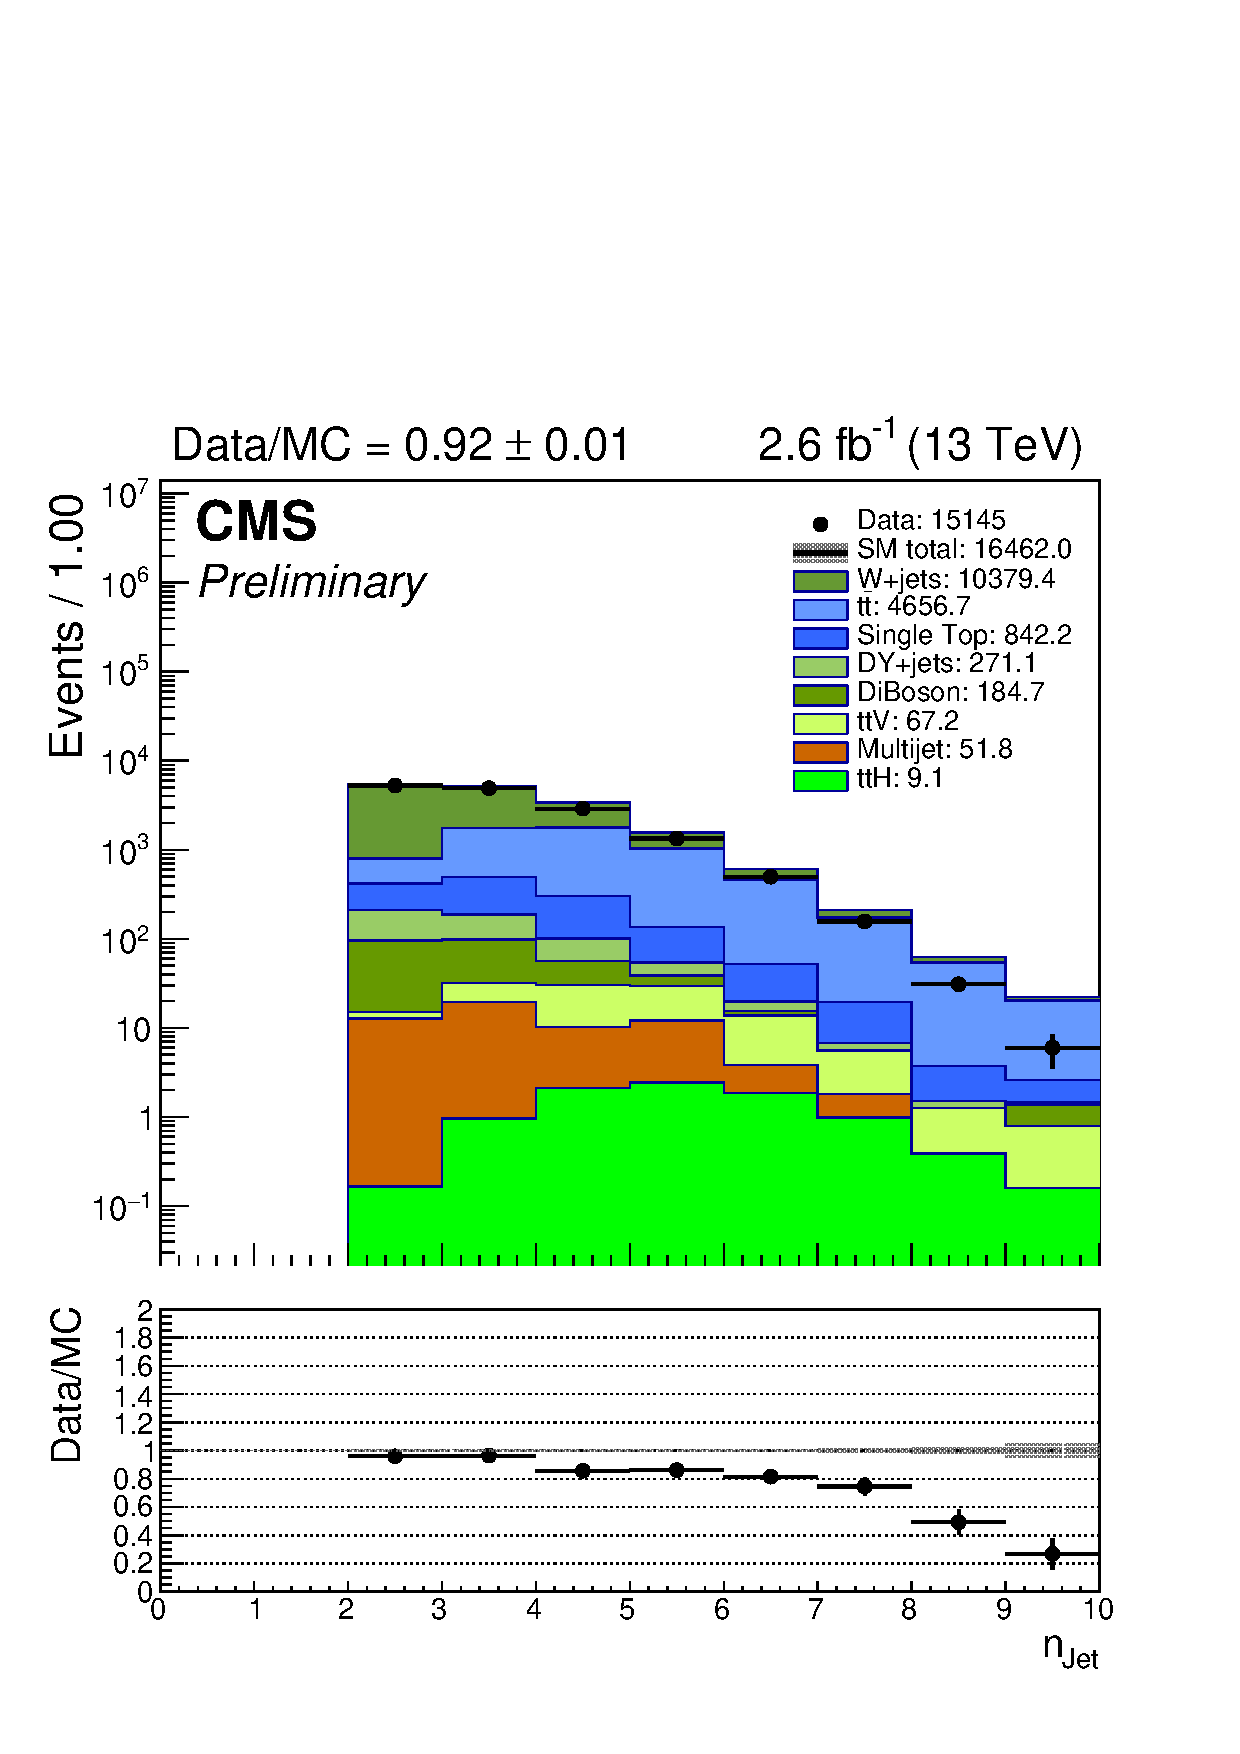
\includegraphics[width=0.5\textwidth]{figures/distributions/Signal/nJet40_sym.pdf}} ~~
%        \subfigure {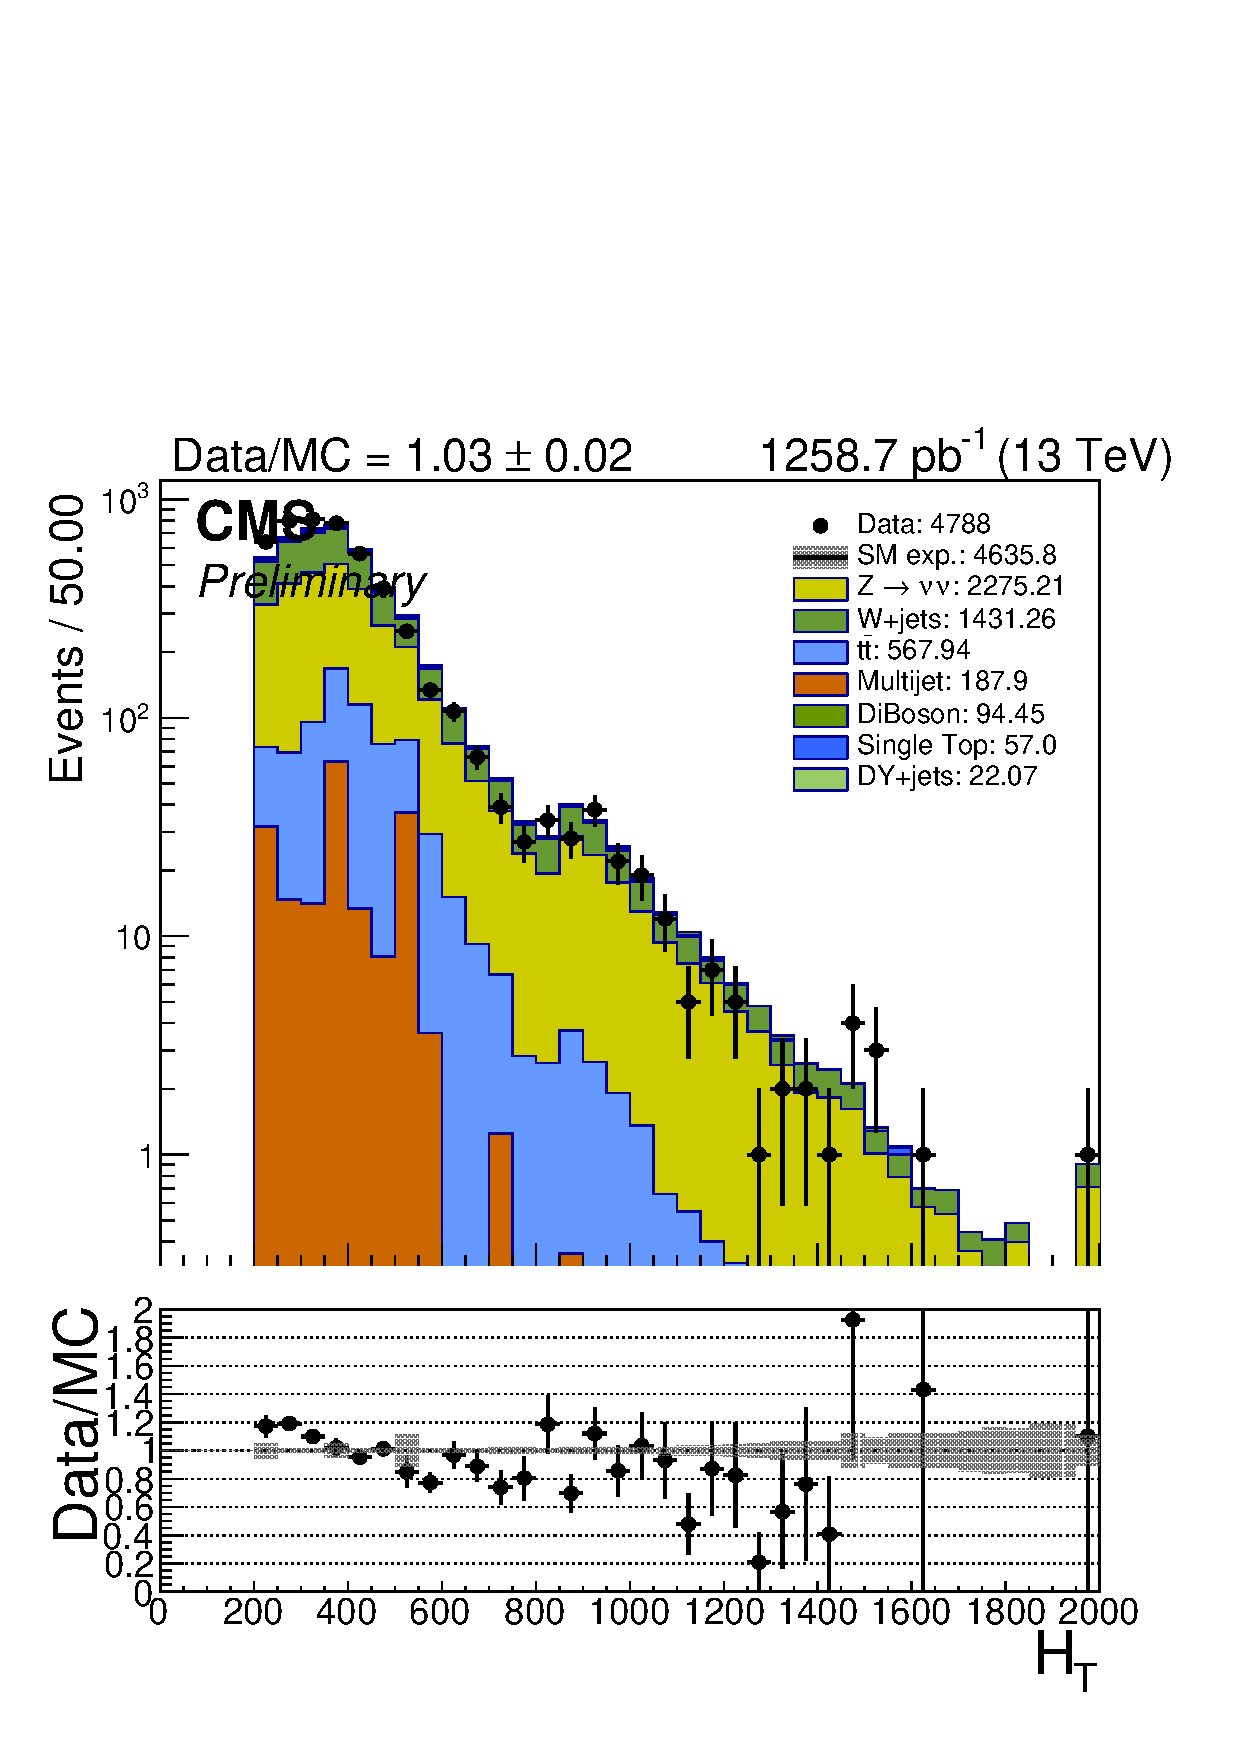
\includegraphics[width=0.5\textwidth]{figures/distributions/Signal/ht40_sym.pdf}} \\
%        \subfigure {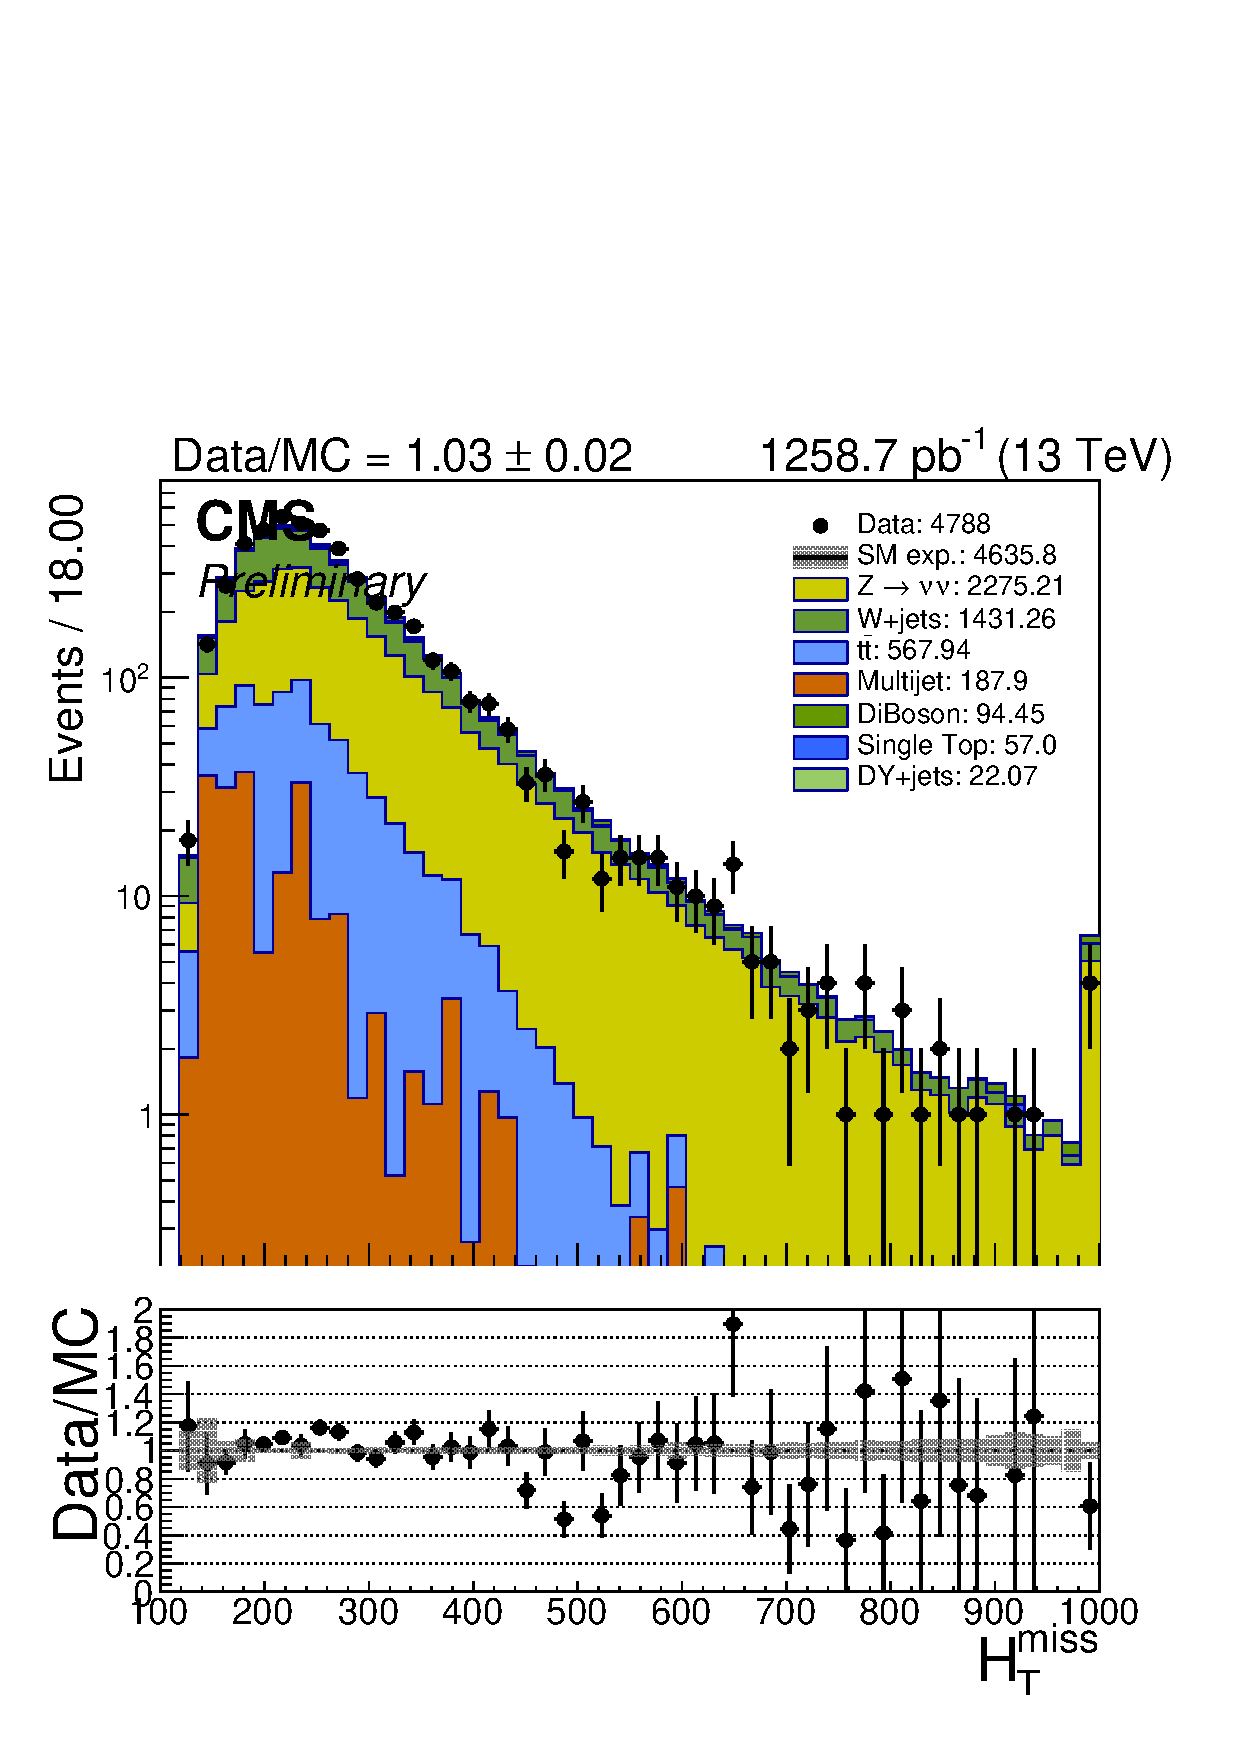
\includegraphics[width=0.5\textwidth]{figures/distributions/Signal/mht40_pt_sym.pdf}} ~~
%        \subfigure {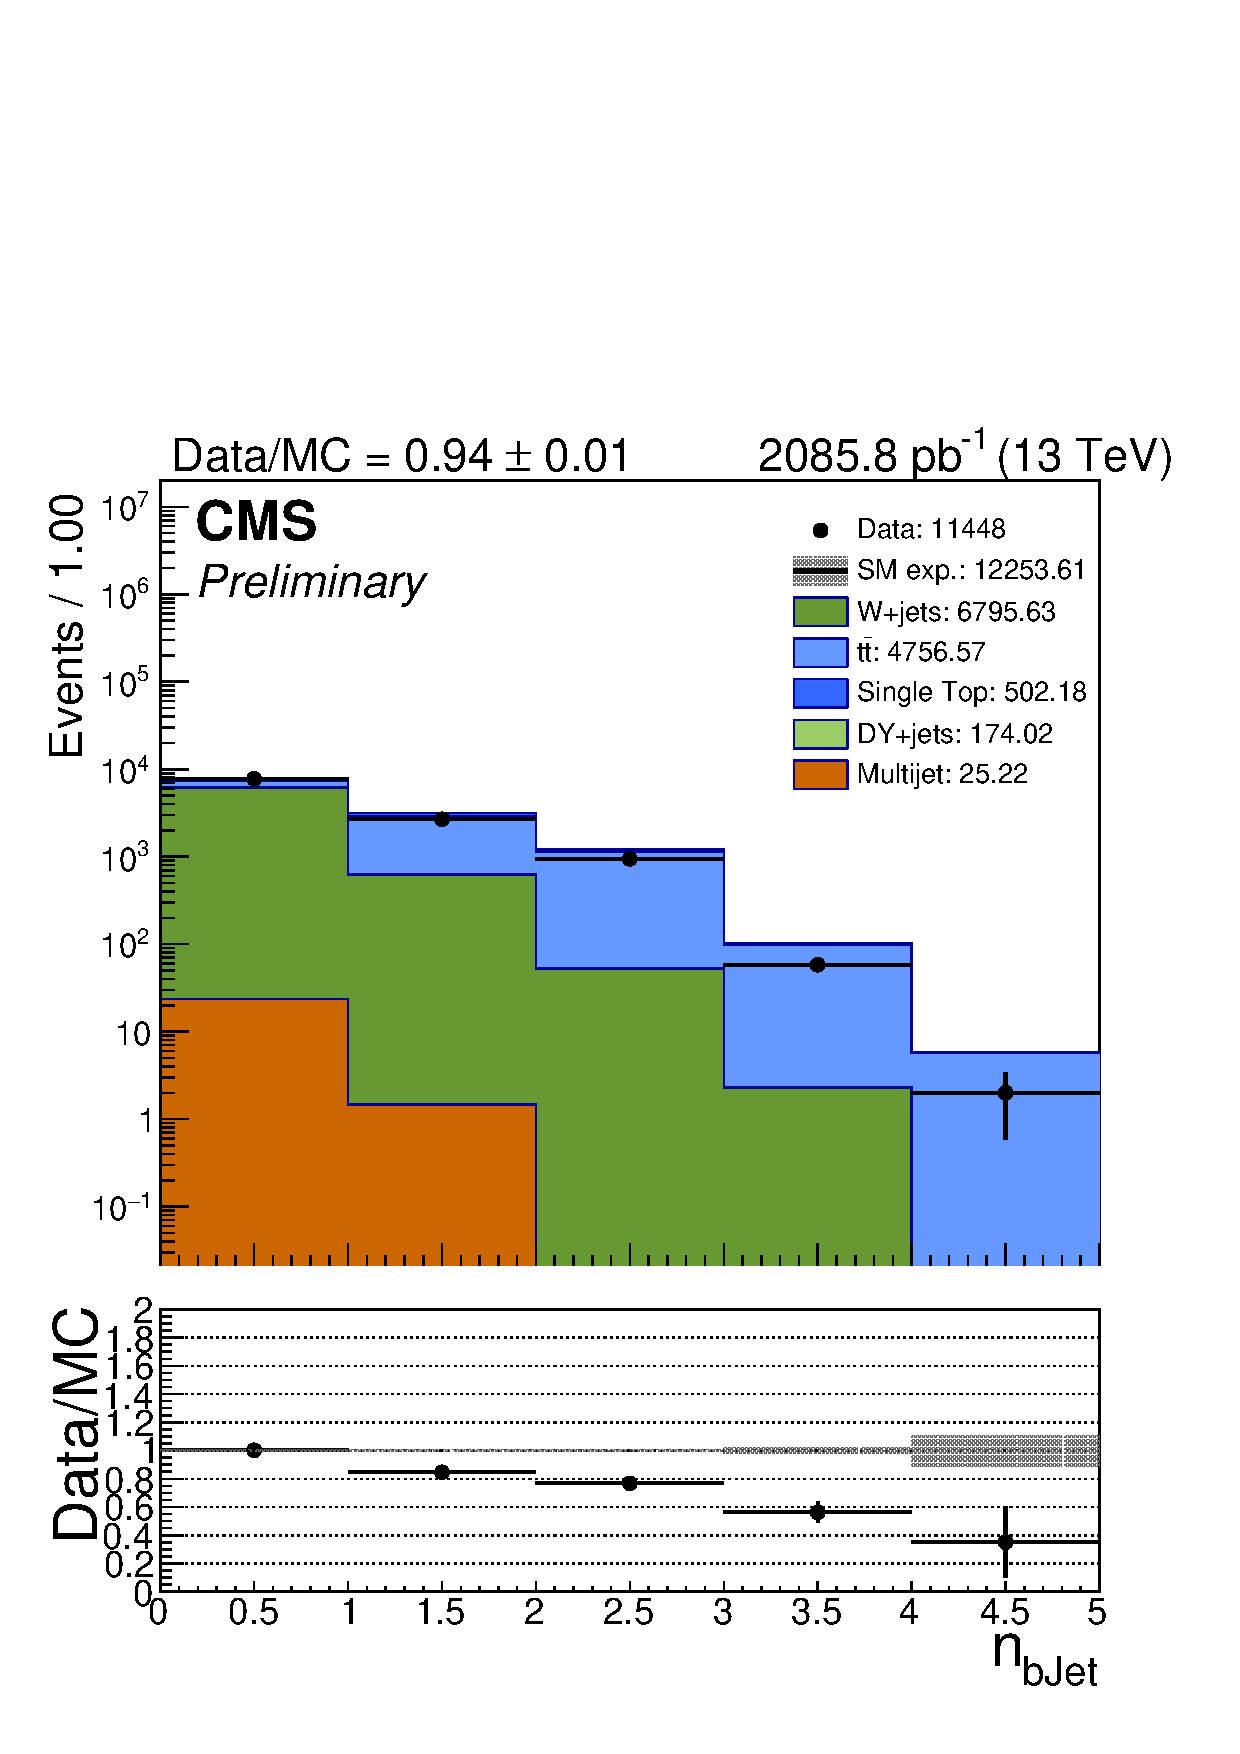
\includegraphics[width=0.5\textwidth]{figures/distributions/Signal/nBJetMedium40_sym.pdf}} \\
%        \caption{Key analysis variables for hadronic signal region (symmetric \njet bins)}
%        \label{fig:distribution_signal_sym}
%    \end{center}
%\end{figure}

%\clearpage
%\begin{figure}
%    \begin{center}
%        \subfigure {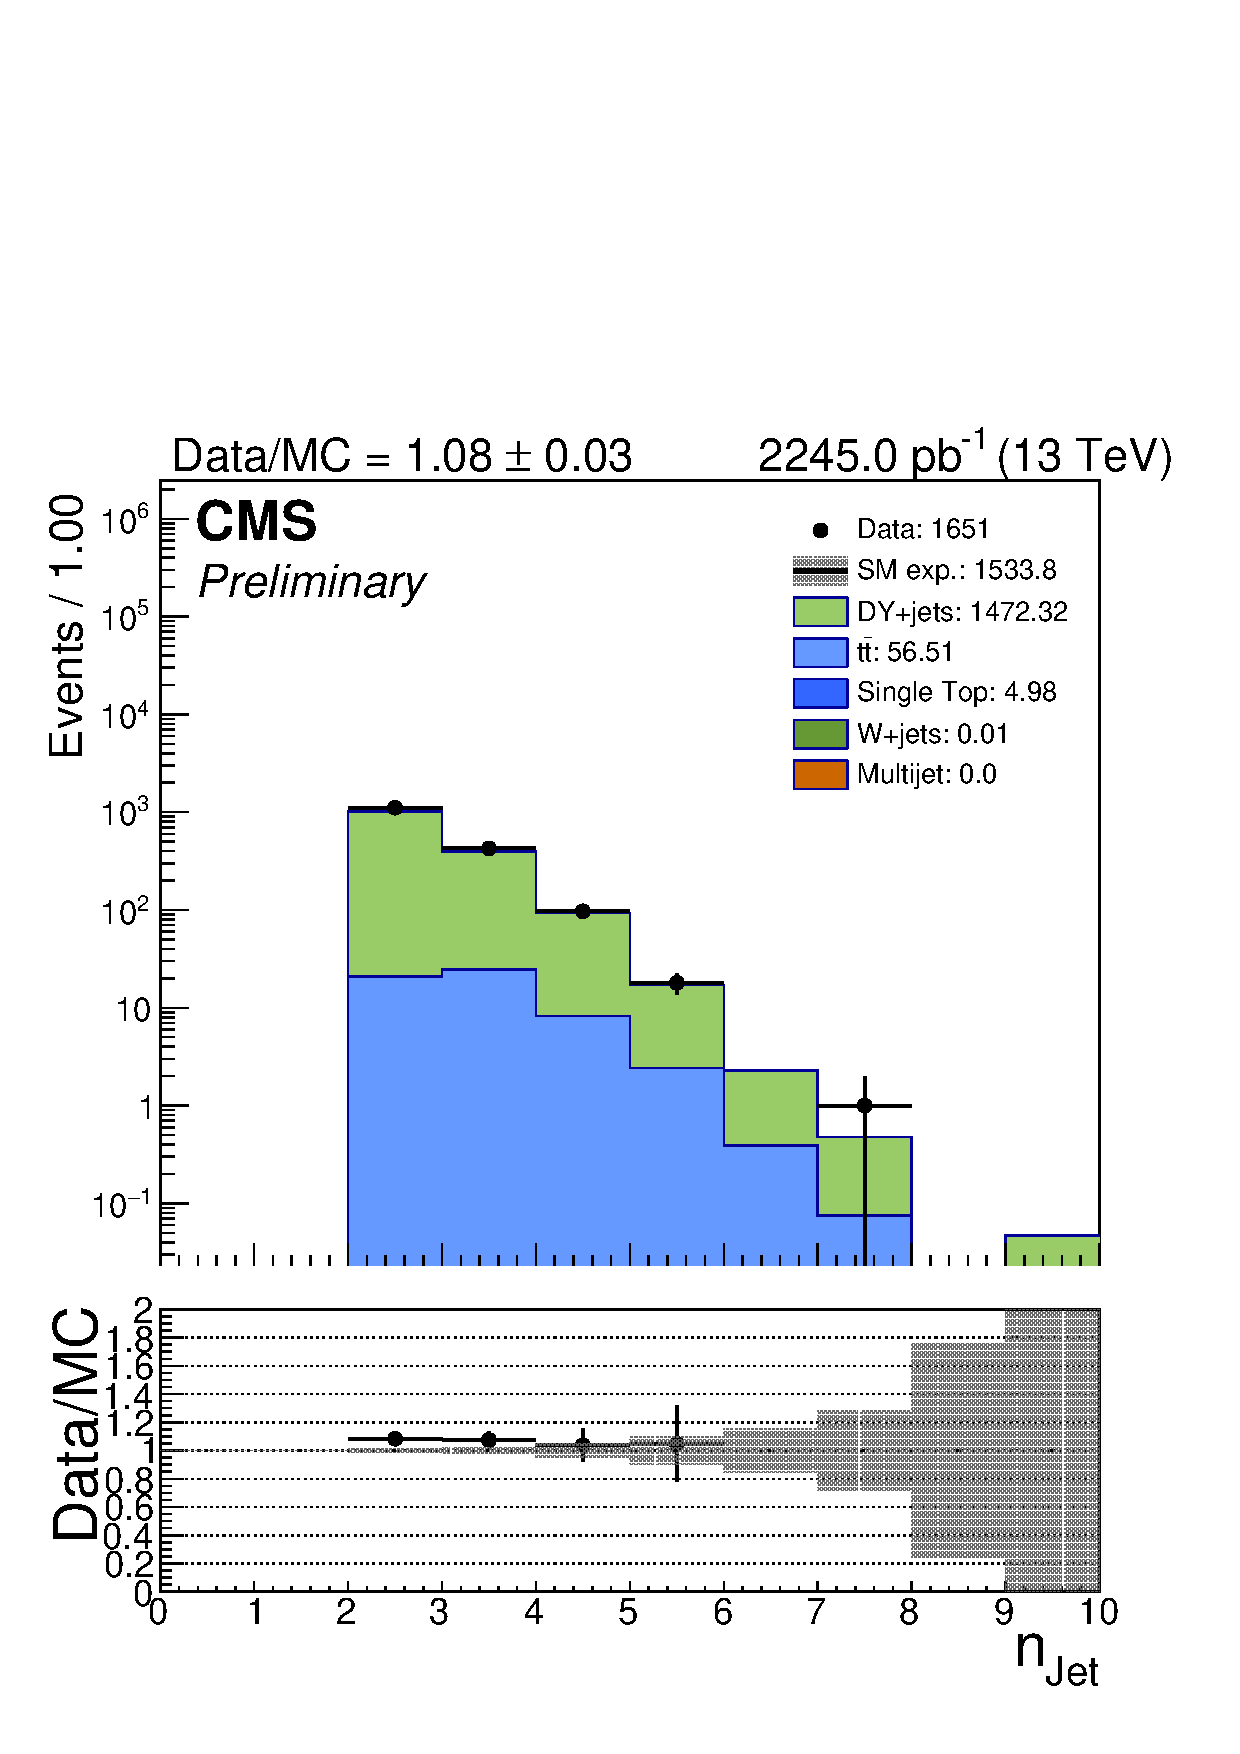
\includegraphics[width=0.5\textwidth]{figures/distributions/Signal/nJet40_asym.pdf}} ~~
%        \subfigure {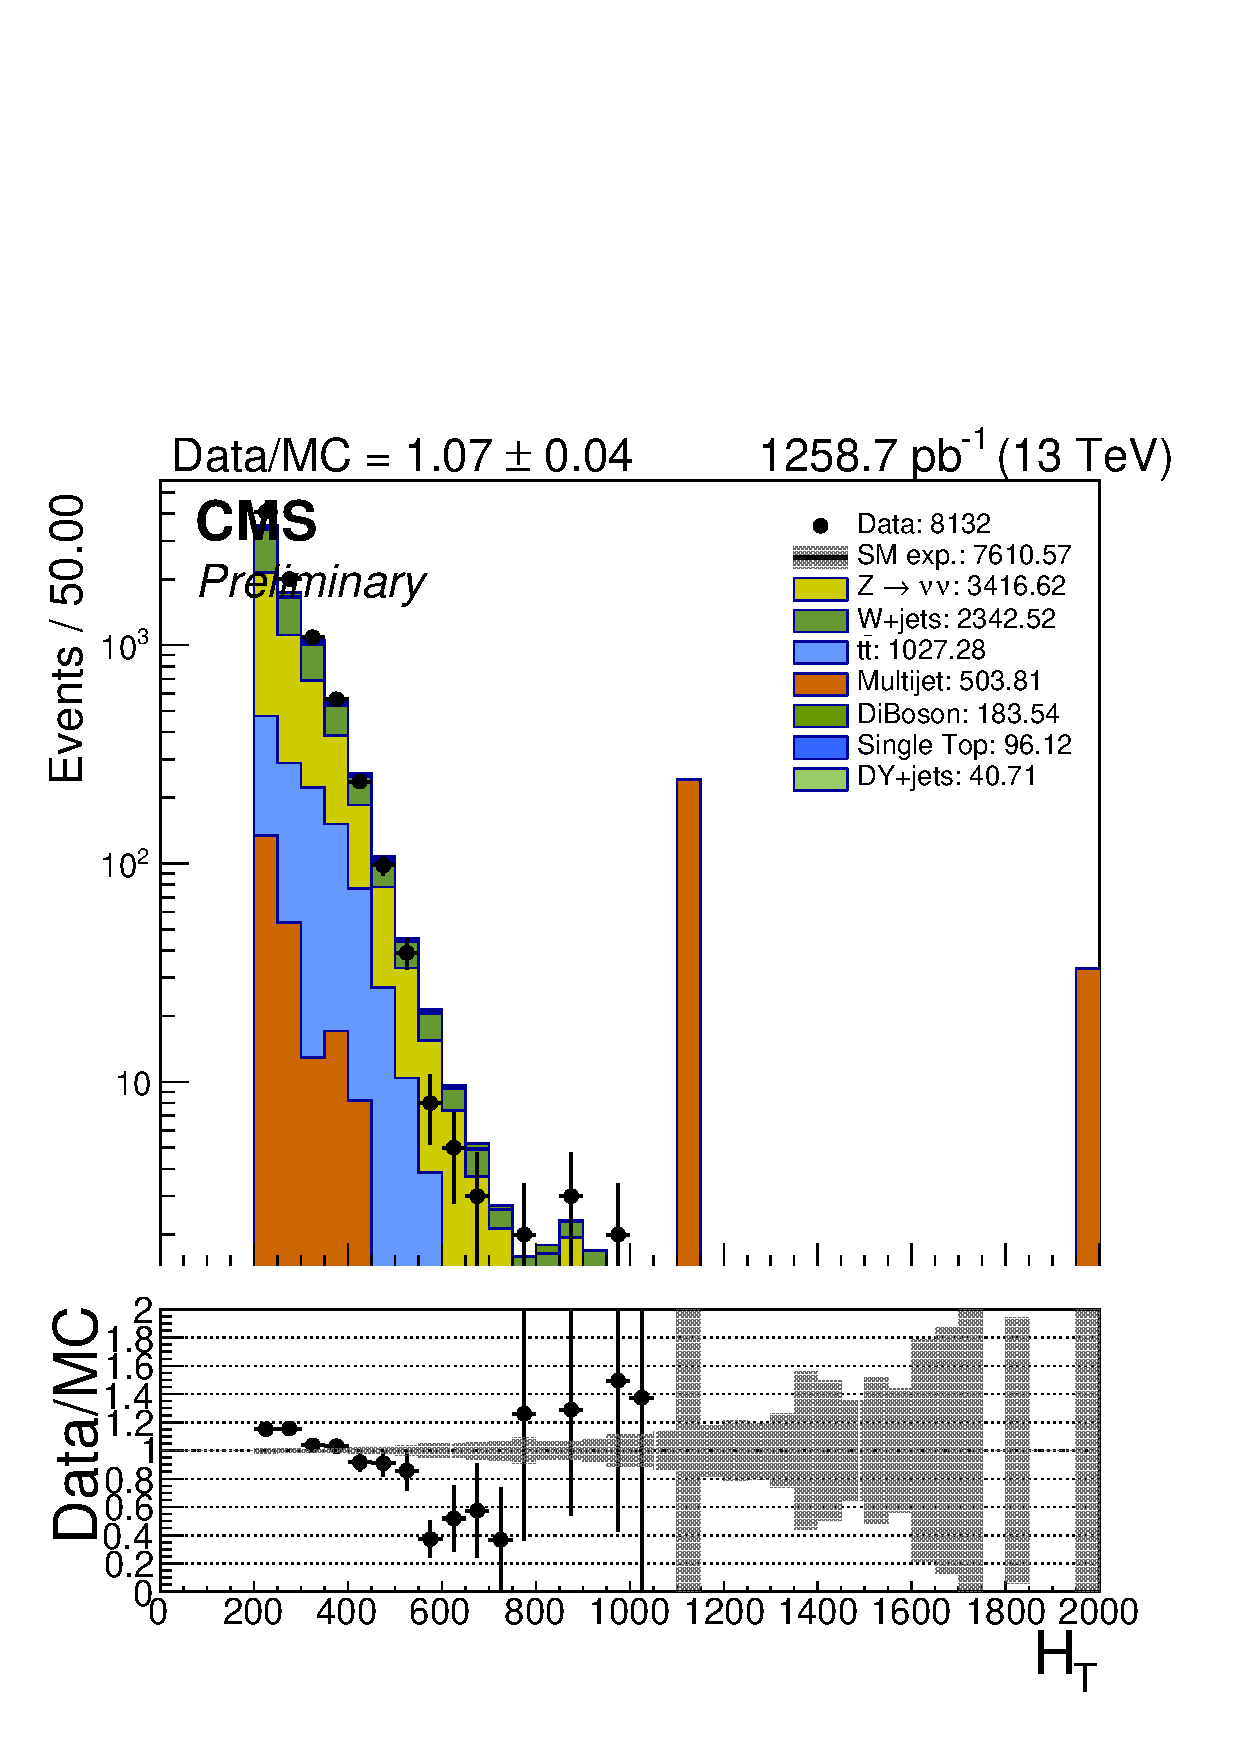
\includegraphics[width=0.5\textwidth]{figures/distributions/Signal/ht40_asym.pdf}} \\
%        \subfigure {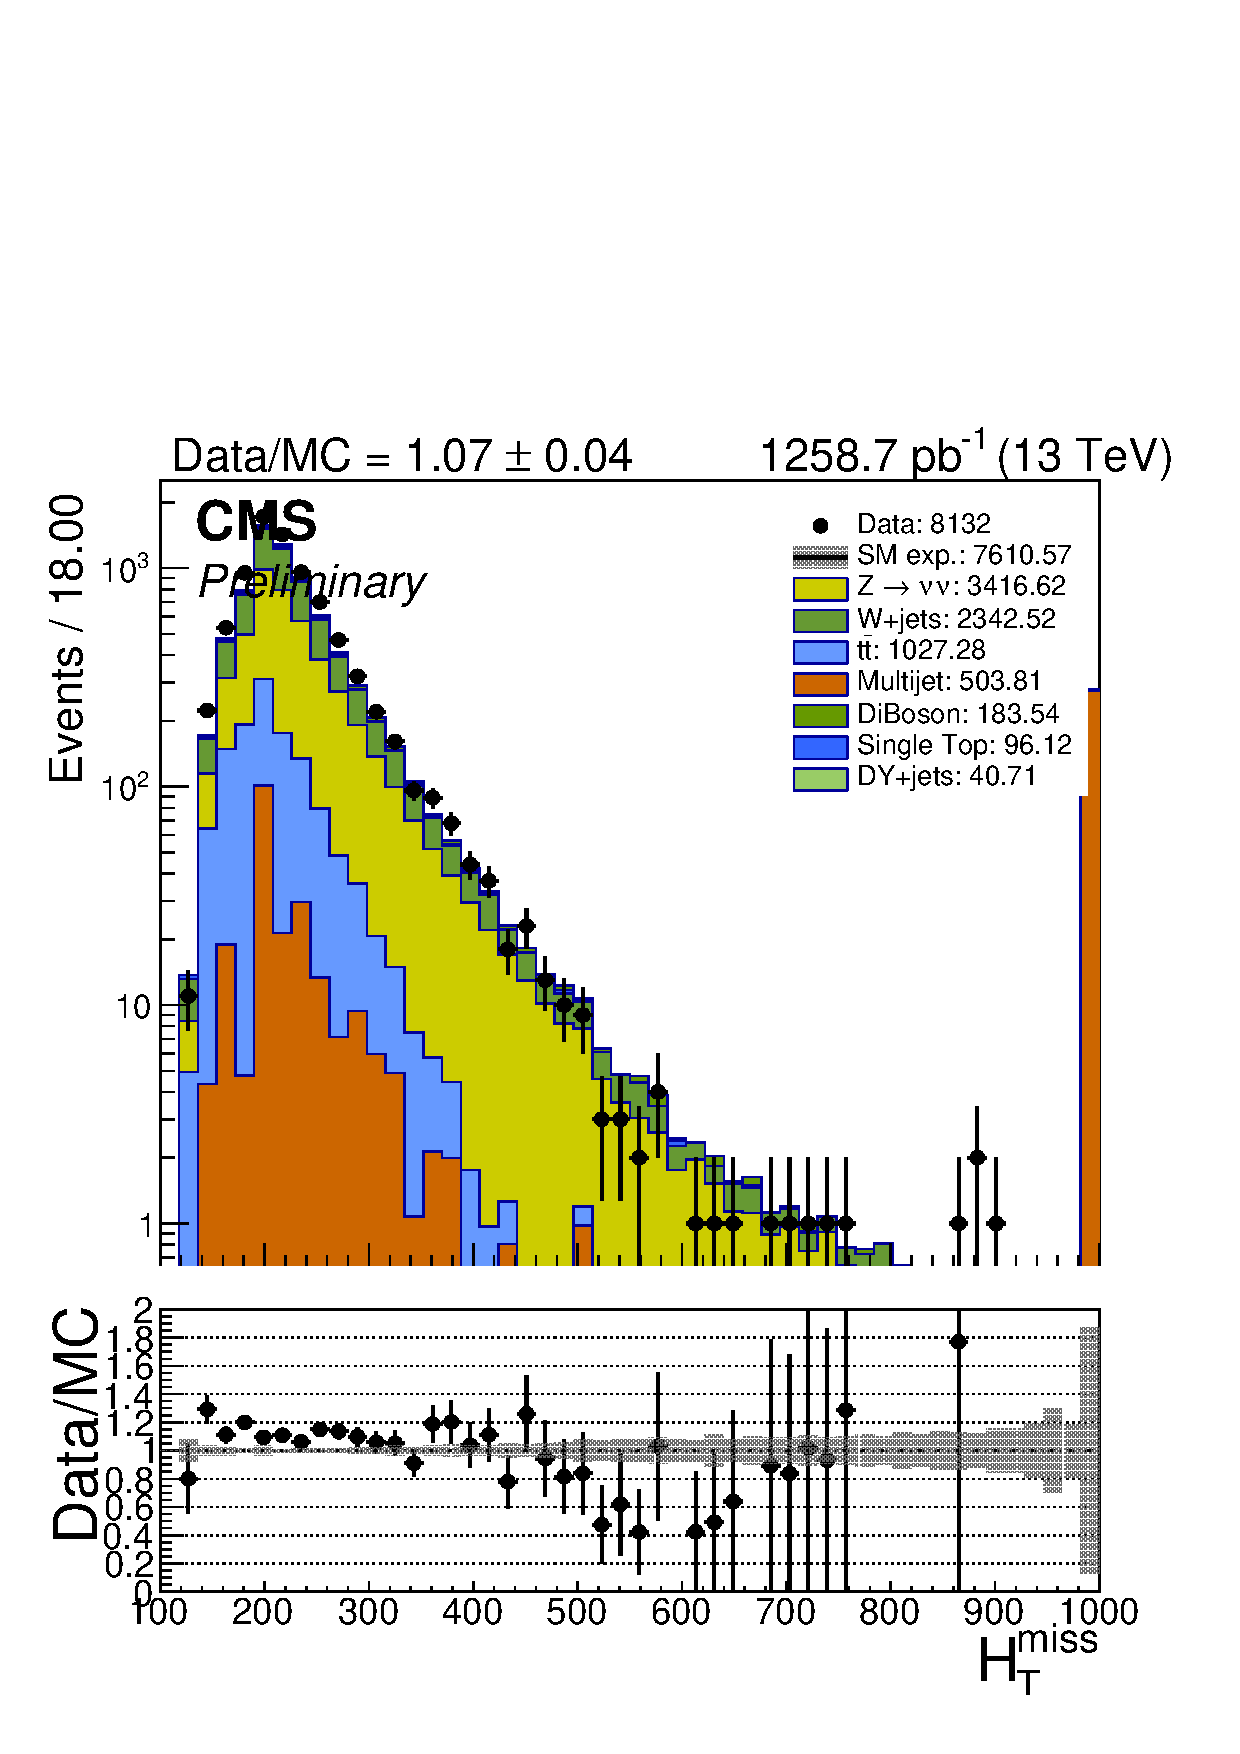
\includegraphics[width=0.5\textwidth]{figures/distributions/Signal/mht40_pt_asym.pdf}} ~~
%        \subfigure {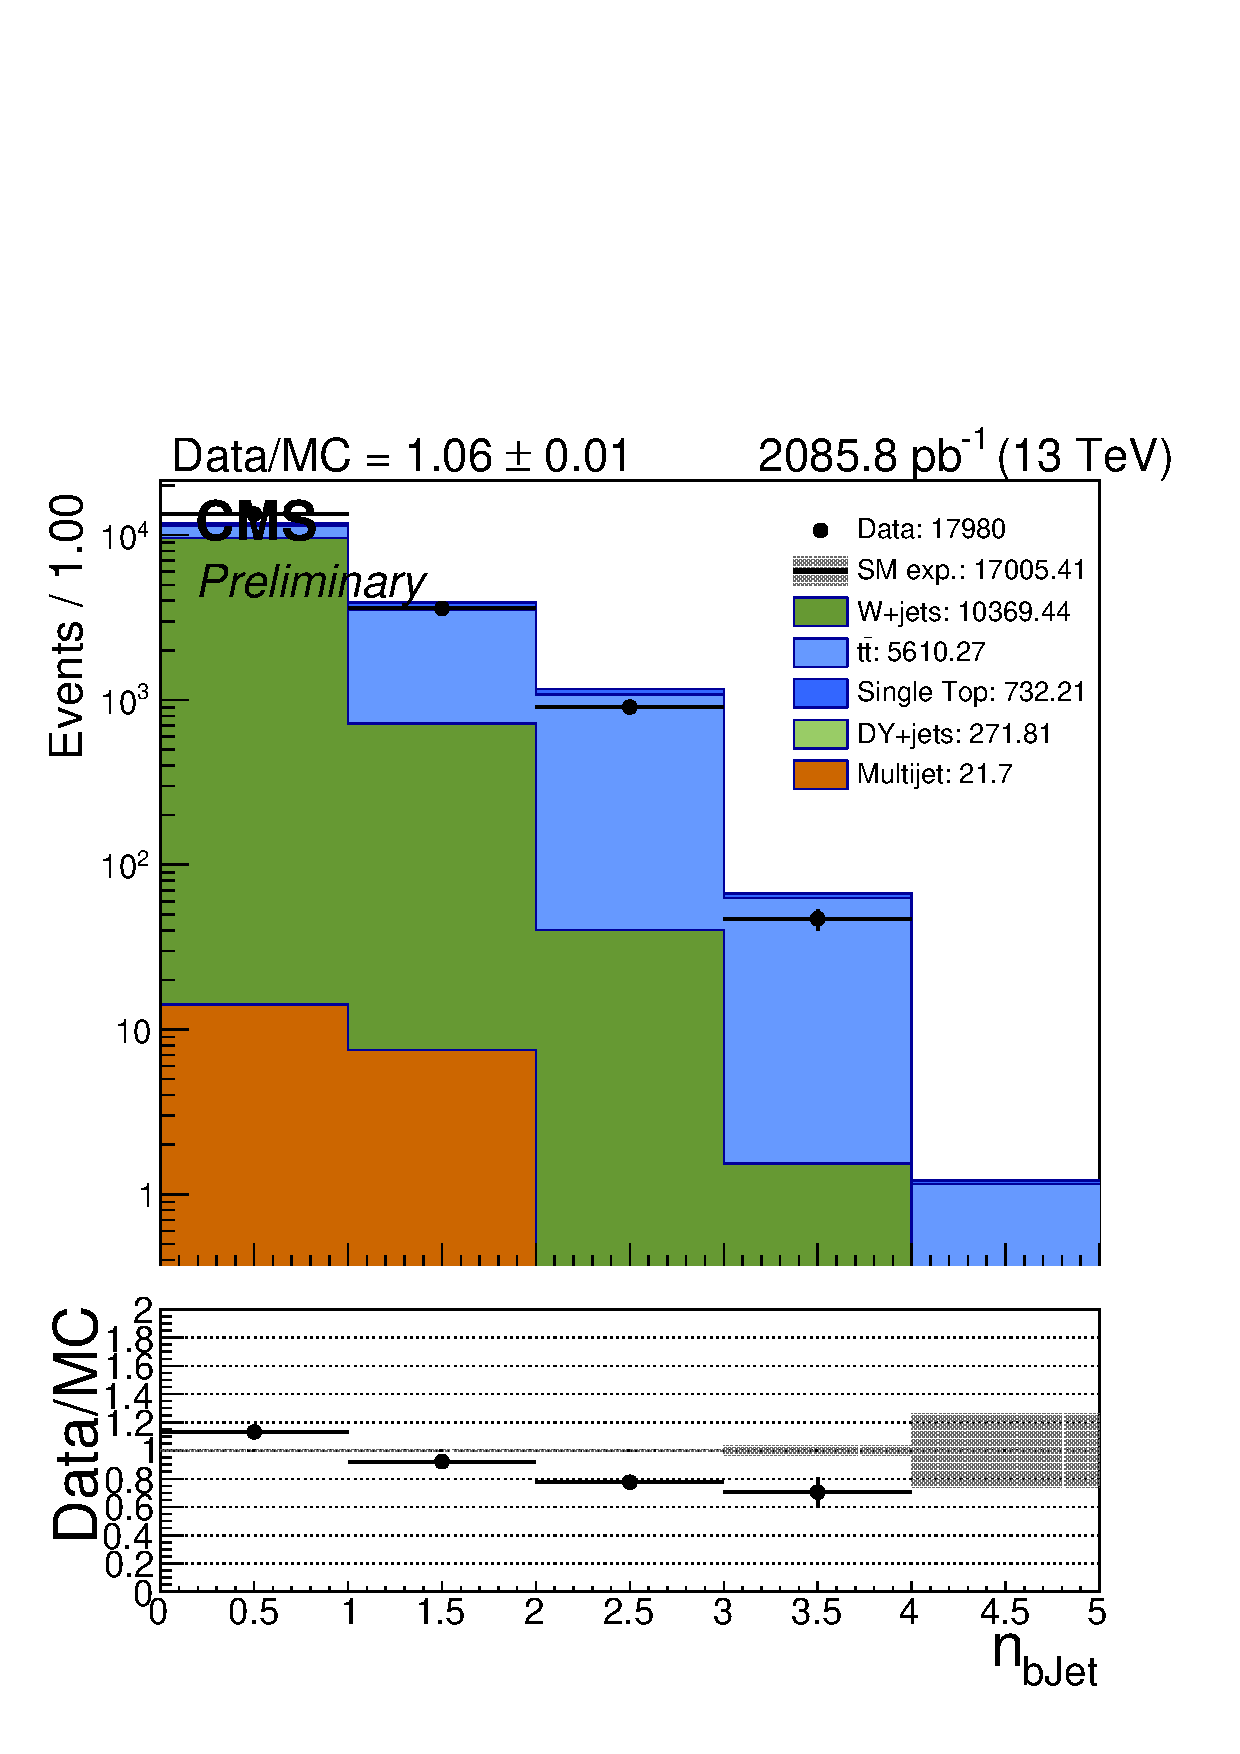
\includegraphics[width=0.5\textwidth]{figures/distributions/Signal/nBJetMedium40_asym.pdf}} \\
%        \caption{Key analysis variables for hadronic signal region (asymmetric \njet bins)}
%        \label{fig:distribution_signal_asym}
%    \end{center}
%\end{figure}

%\clearpage
%\begin{figure}
%    \begin{center}
%        \subfigure {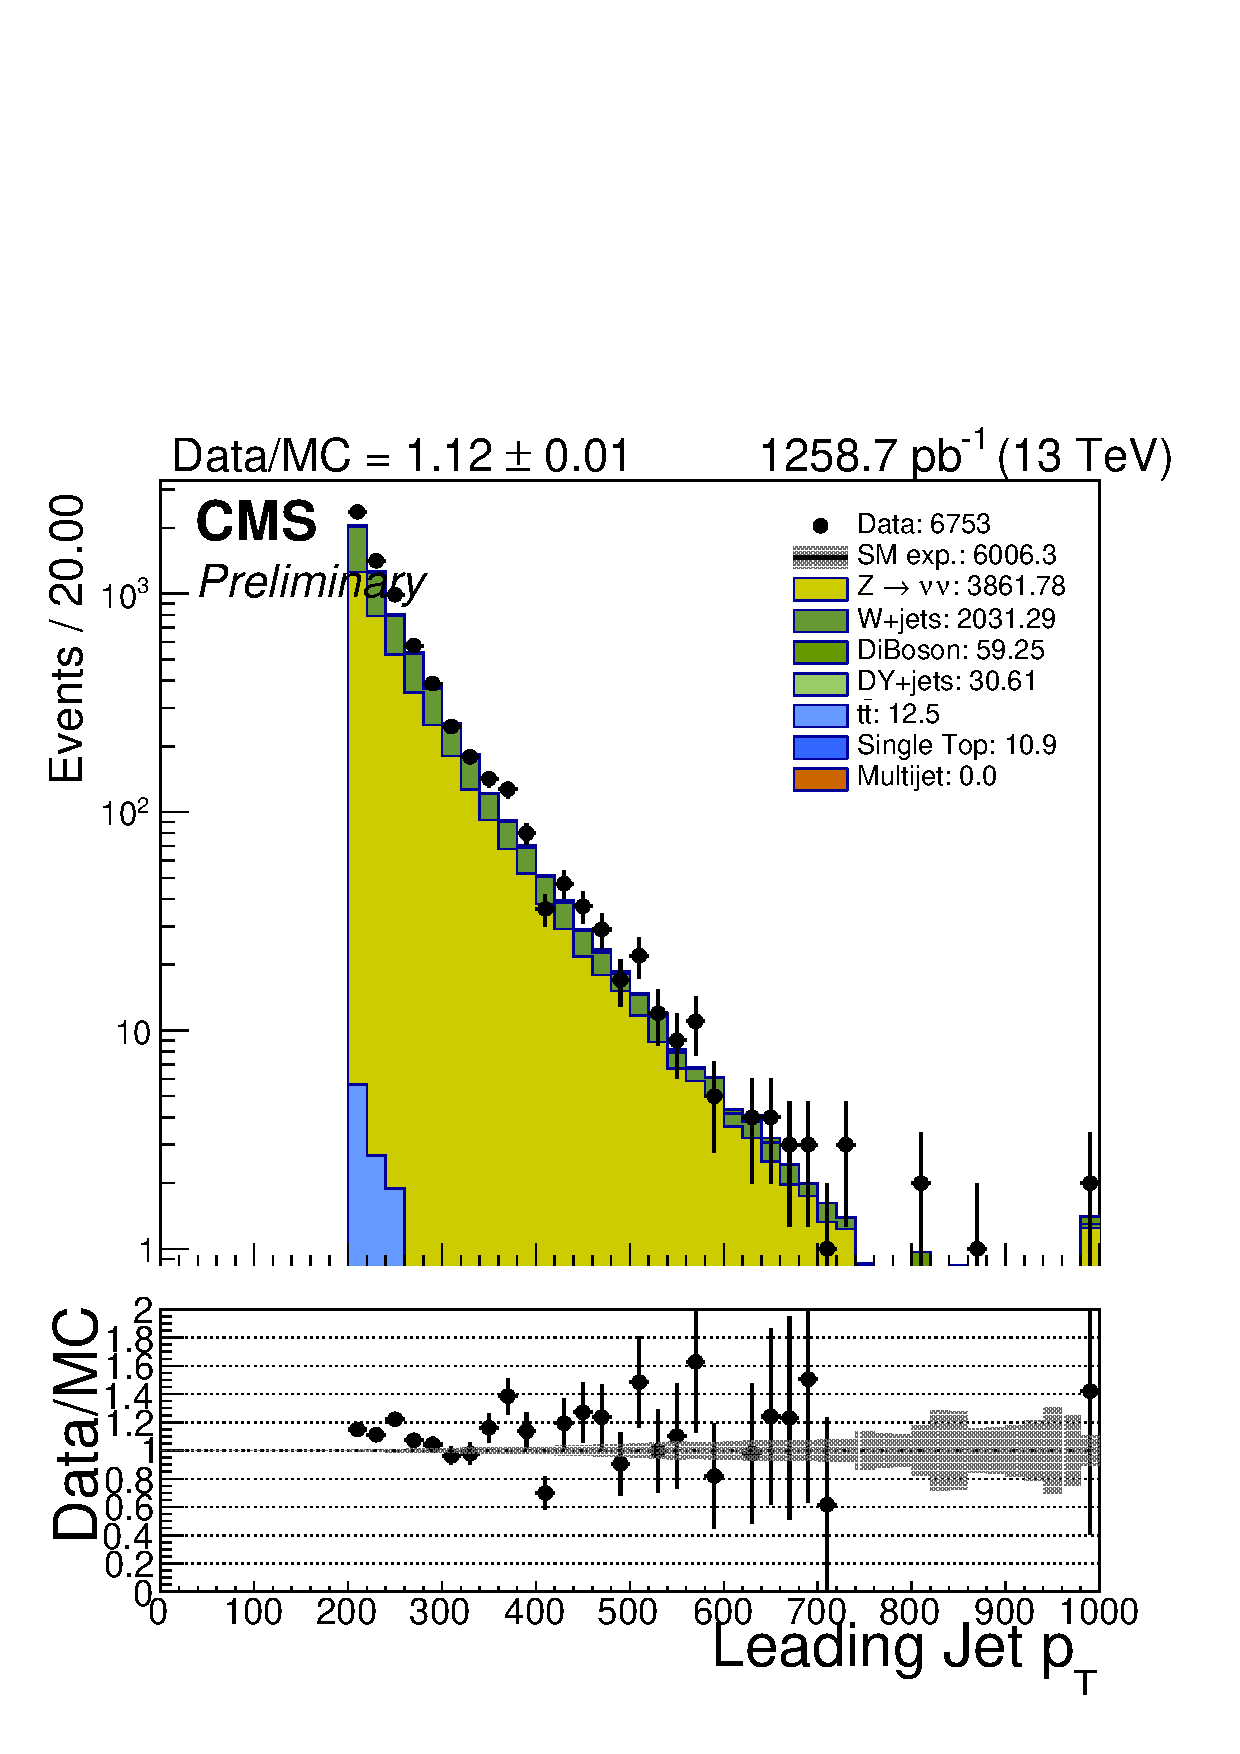
\includegraphics[width=0.5\textwidth]{figures/distributions/Signal/jet_pt[0]_eq1j.pdf}} ~~
%        \subfigure {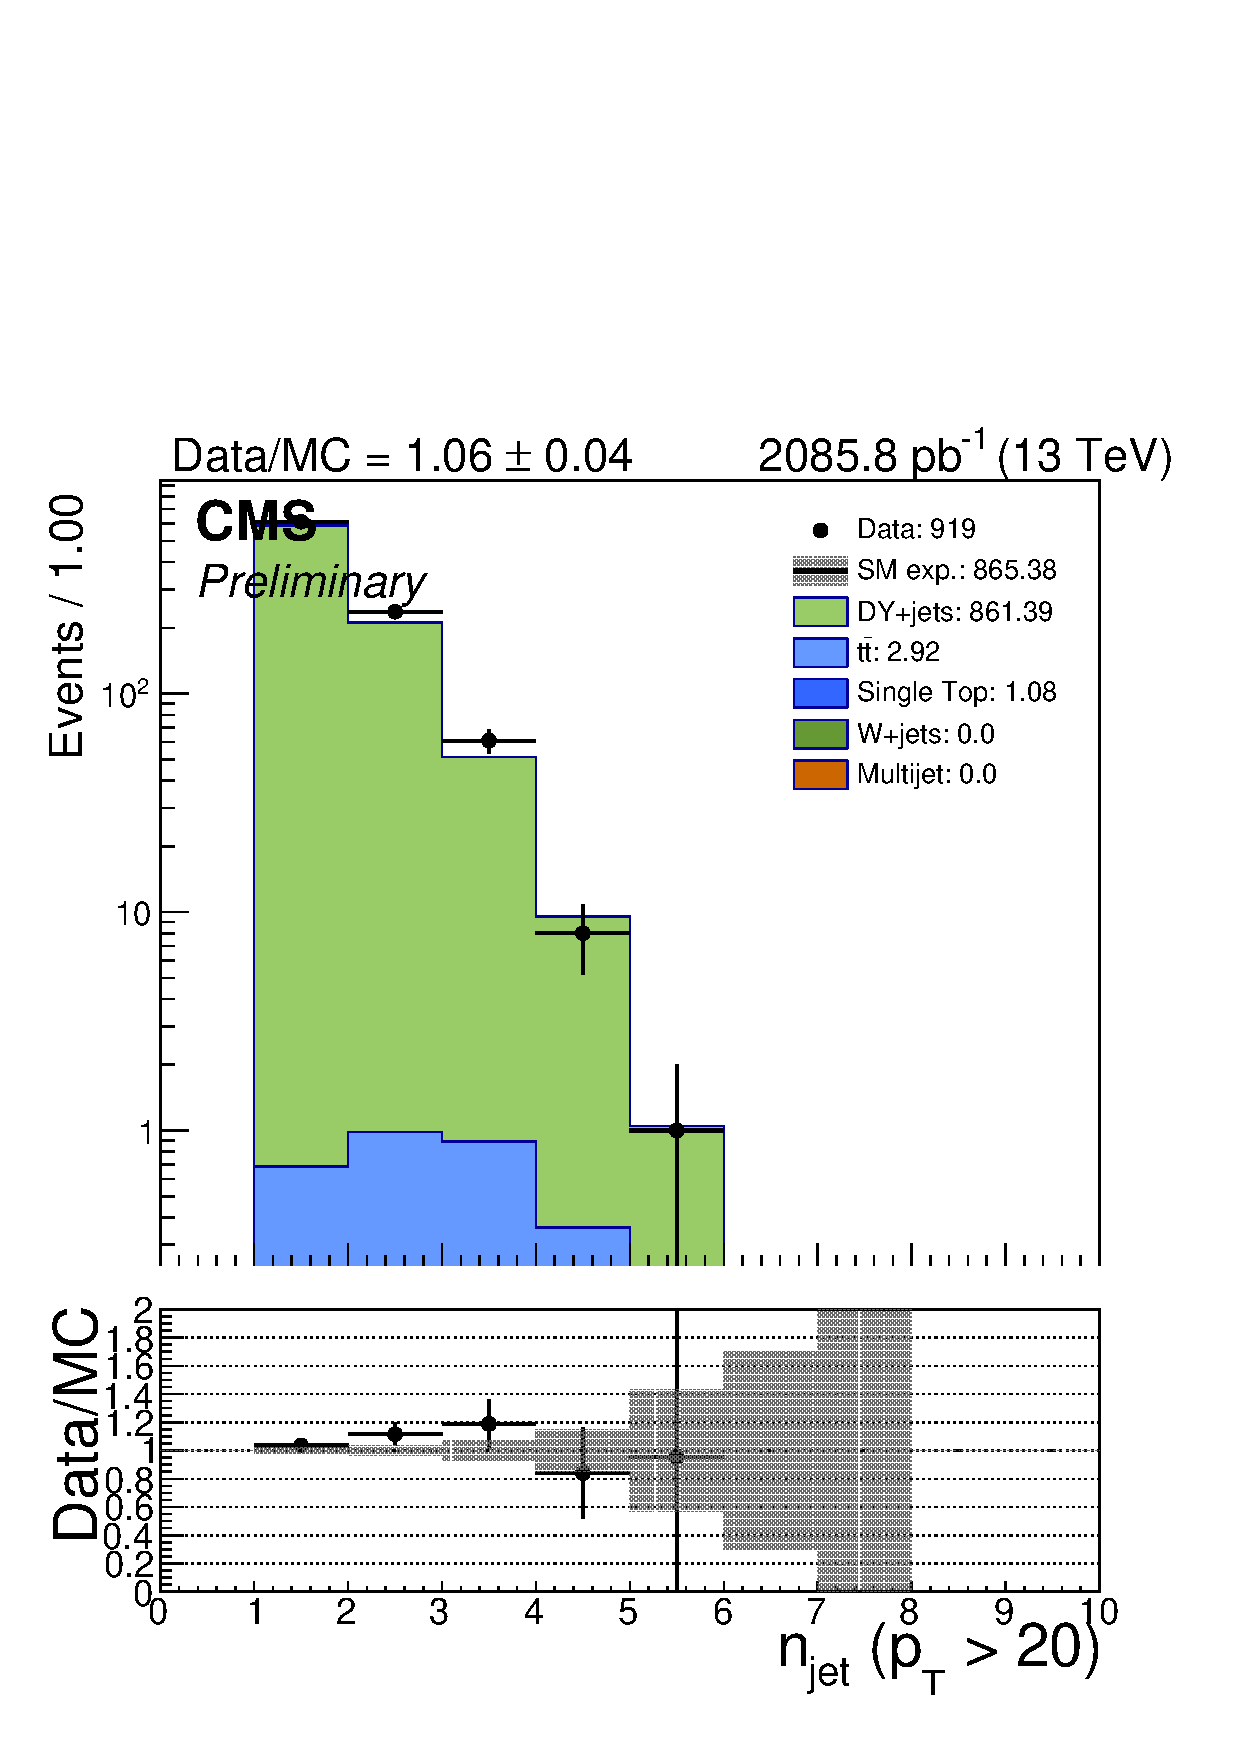
\includegraphics[width=0.5\textwidth]{figures/distributions/Signal/njetInc_eq1j.pdf}} \\
%        \subfigure {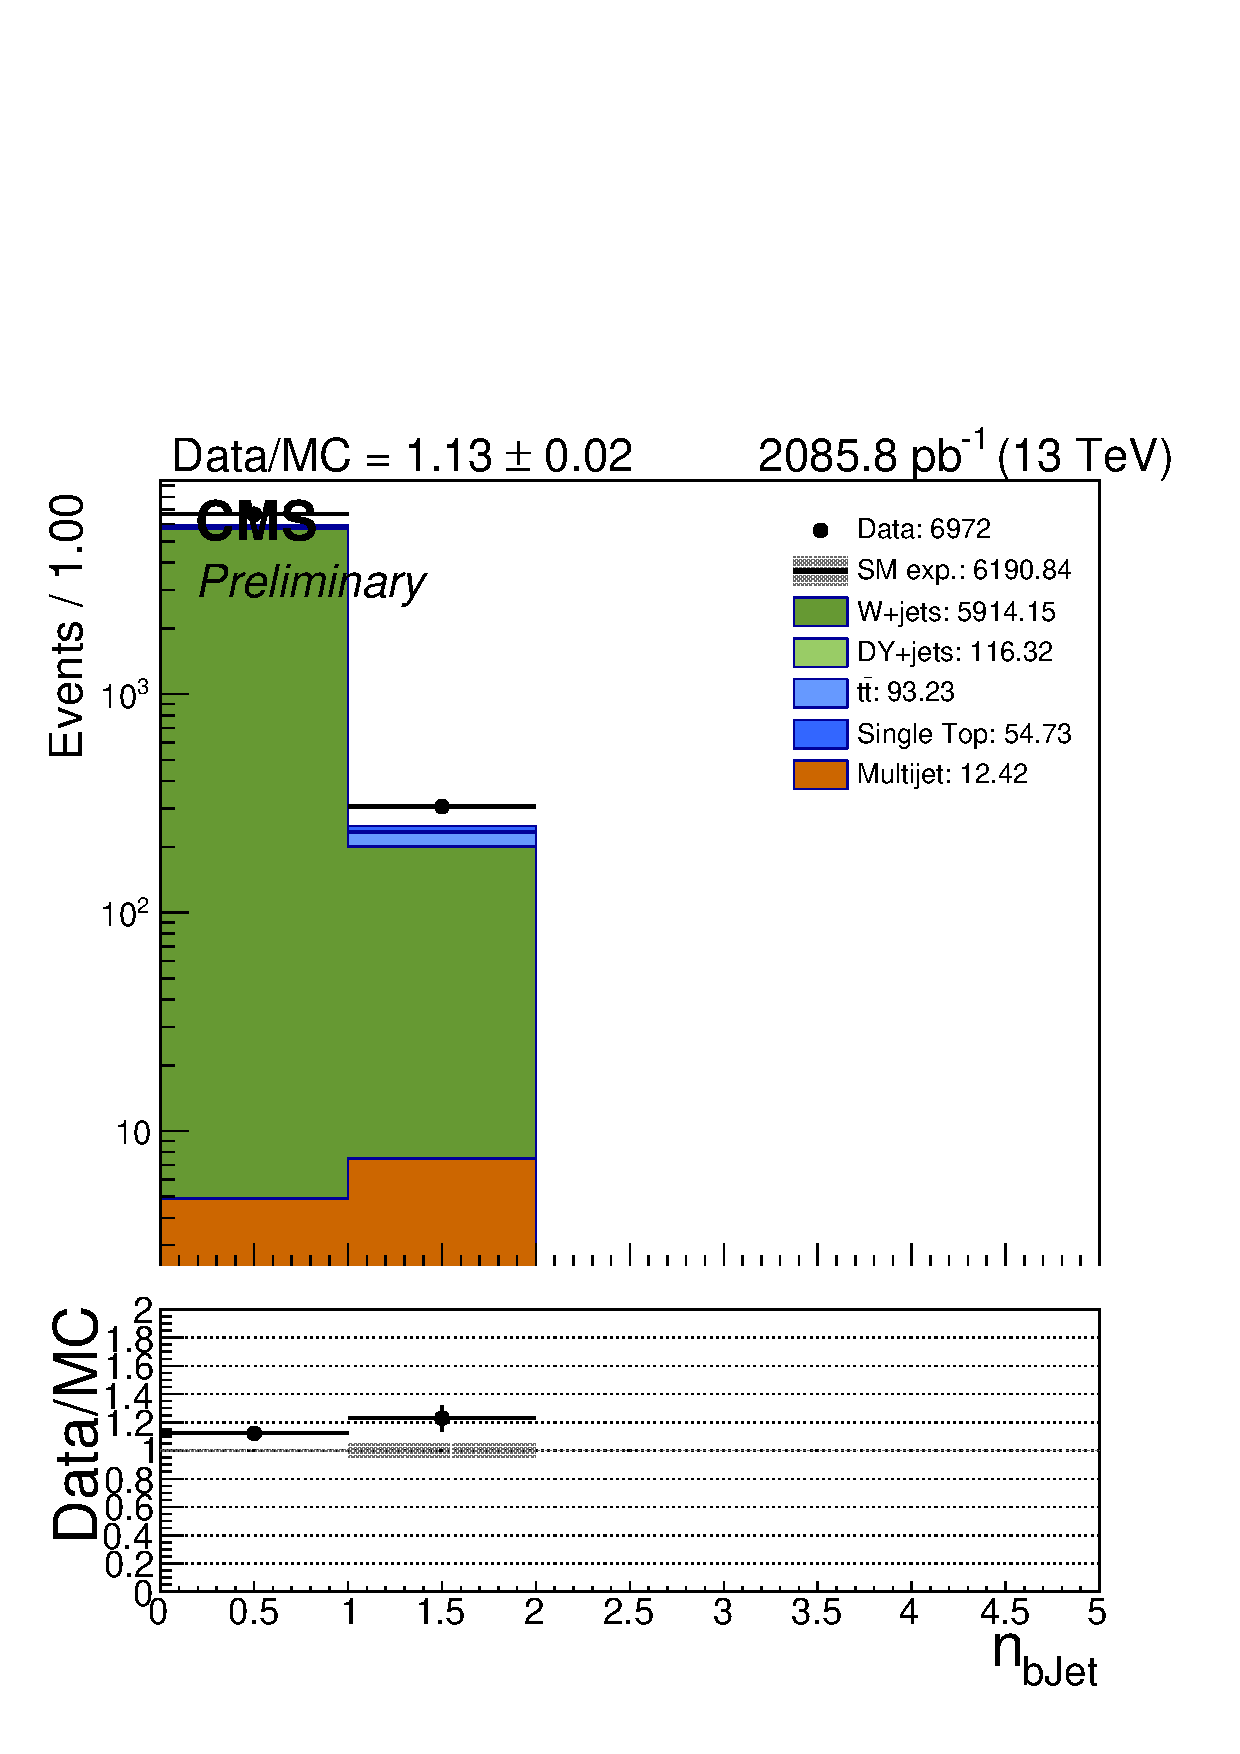
\includegraphics[width=0.5\textwidth]{figures/distributions/Signal/nBJetMedium40_eq1j.pdf}} ~~
%        \subfigure {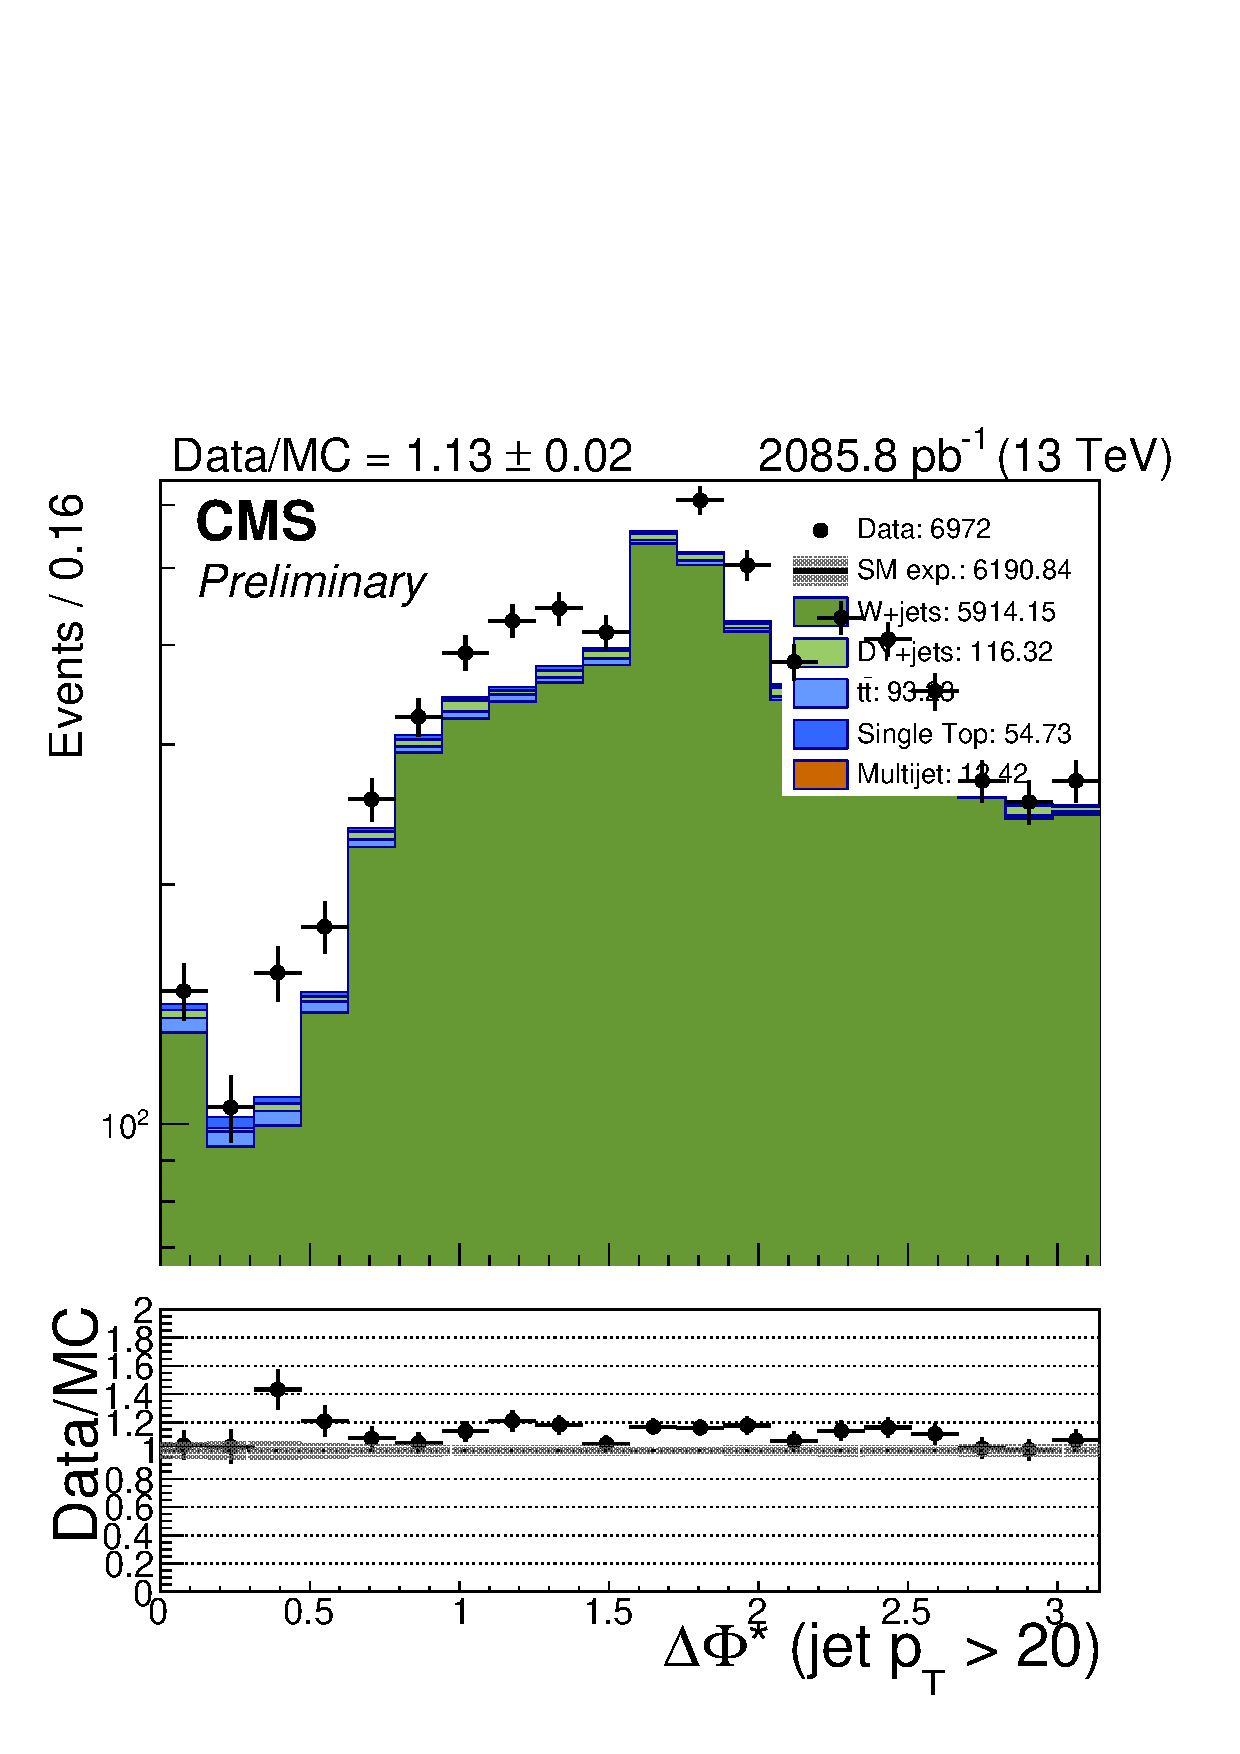
\includegraphics[width=0.5\textwidth]{figures/distributions/Signal/biasedDPhiInc_eq1j.pdf}} \\
%        \caption{Key analysis variables for hadronic signal region (monojet bins)}
%        \label{fig:distribution_signal_mono}
%    \end{center}
%\end{figure}



